% Options for packages loaded elsewhere
% Options for packages loaded elsewhere
\PassOptionsToPackage{unicode}{hyperref}
\PassOptionsToPackage{hyphens}{url}
\PassOptionsToPackage{dvipsnames,svgnames,x11names}{xcolor}
%
\documentclass[
  number,
  preprint,
  onecolumn]{elsarticle}
\usepackage{xcolor}
\usepackage{amsmath,amssymb}
\setcounter{secnumdepth}{5}
\usepackage{iftex}
\ifPDFTeX
  \usepackage[T1]{fontenc}
  \usepackage[utf8]{inputenc}
  \usepackage{textcomp} % provide euro and other symbols
\else % if luatex or xetex
  \usepackage{unicode-math} % this also loads fontspec
  \defaultfontfeatures{Scale=MatchLowercase}
  \defaultfontfeatures[\rmfamily]{Ligatures=TeX,Scale=1}
\fi
\usepackage{lmodern}
\ifPDFTeX\else
  % xetex/luatex font selection
\fi
% Use upquote if available, for straight quotes in verbatim environments
\IfFileExists{upquote.sty}{\usepackage{upquote}}{}
\IfFileExists{microtype.sty}{% use microtype if available
  \usepackage[]{microtype}
  \UseMicrotypeSet[protrusion]{basicmath} % disable protrusion for tt fonts
}{}
\makeatletter
\@ifundefined{KOMAClassName}{% if non-KOMA class
  \IfFileExists{parskip.sty}{%
    \usepackage{parskip}
  }{% else
    \setlength{\parindent}{0pt}
    \setlength{\parskip}{6pt plus 2pt minus 1pt}}
}{% if KOMA class
  \KOMAoptions{parskip=half}}
\makeatother
% Make \paragraph and \subparagraph free-standing
\makeatletter
\ifx\paragraph\undefined\else
  \let\oldparagraph\paragraph
  \renewcommand{\paragraph}{
    \@ifstar
      \xxxParagraphStar
      \xxxParagraphNoStar
  }
  \newcommand{\xxxParagraphStar}[1]{\oldparagraph*{#1}\mbox{}}
  \newcommand{\xxxParagraphNoStar}[1]{\oldparagraph{#1}\mbox{}}
\fi
\ifx\subparagraph\undefined\else
  \let\oldsubparagraph\subparagraph
  \renewcommand{\subparagraph}{
    \@ifstar
      \xxxSubParagraphStar
      \xxxSubParagraphNoStar
  }
  \newcommand{\xxxSubParagraphStar}[1]{\oldsubparagraph*{#1}\mbox{}}
  \newcommand{\xxxSubParagraphNoStar}[1]{\oldsubparagraph{#1}\mbox{}}
\fi
\makeatother


\usepackage{longtable,booktabs,array}
\newcounter{none} % for unnumbered tables
\usepackage{calc} % for calculating minipage widths
% Correct order of tables after \paragraph or \subparagraph
\usepackage{etoolbox}
\makeatletter
\patchcmd\longtable{\par}{\if@noskipsec\mbox{}\fi\par}{}{}
\makeatother
% Allow footnotes in longtable head/foot
\IfFileExists{footnotehyper.sty}{\usepackage{footnotehyper}}{\usepackage{footnote}}
\makesavenoteenv{longtable}
\usepackage{graphicx}
\makeatletter
\newsavebox\pandoc@box
\newcommand*\pandocbounded[1]{% scales image to fit in text height/width
  \sbox\pandoc@box{#1}%
  \Gscale@div\@tempa{\textheight}{\dimexpr\ht\pandoc@box+\dp\pandoc@box\relax}%
  \Gscale@div\@tempb{\linewidth}{\wd\pandoc@box}%
  \ifdim\@tempb\p@<\@tempa\p@\let\@tempa\@tempb\fi% select the smaller of both
  \ifdim\@tempa\p@<\p@\scalebox{\@tempa}{\usebox\pandoc@box}%
  \else\usebox{\pandoc@box}%
  \fi%
}
% Set default figure placement to htbp
\def\fps@figure{htbp}
\makeatother





\setlength{\emergencystretch}{3em} % prevent overfull lines

\providecommand{\tightlist}{%
  \setlength{\itemsep}{0pt}\setlength{\parskip}{0pt}}



 
\usepackage[]{natbib}
\bibliographystyle{elsarticle-num}


\usepackage{lineno}
\linenumbers
\makeatletter
\@ifpackageloaded{float}{}{\usepackage{float}}
\floatstyle{plain}
\@ifundefined{c@chapter}{\newfloat{suppfig}{h}{losfig}}{\newfloat{suppfig}{h}{losfig}[chapter]}
\floatname{suppfig}{Supp. Figure}
\newcommand*\listofsuppfigs{\listof{suppfig}{List of Supp. Figures}}
\makeatother
\makeatletter
\@ifpackageloaded{float}{}{\usepackage{float}}
\floatstyle{plain}
\@ifundefined{c@chapter}{\newfloat{supptable}{h}{lostab}}{\newfloat{supptable}{h}{lostab}[chapter]}
\floatname{supptable}{Supp. Table}
\newcommand*\listofsupptables{\listof{supptable}{List of Supp. Tables}}
\makeatother
\makeatletter
\@ifpackageloaded{caption}{}{\usepackage{caption}}
\AtBeginDocument{%
\ifdefined\contentsname
  \renewcommand*\contentsname{Table of contents}
\else
  \newcommand\contentsname{Table of contents}
\fi
\ifdefined\listfigurename
  \renewcommand*\listfigurename{List of Figures}
\else
  \newcommand\listfigurename{List of Figures}
\fi
\ifdefined\listtablename
  \renewcommand*\listtablename{List of Tables}
\else
  \newcommand\listtablename{List of Tables}
\fi
\ifdefined\figurename
  \renewcommand*\figurename{Figure}
\else
  \newcommand\figurename{Figure}
\fi
\ifdefined\tablename
  \renewcommand*\tablename{Table}
\else
  \newcommand\tablename{Table}
\fi
}
\@ifpackageloaded{float}{}{\usepackage{float}}
\floatstyle{ruled}
\@ifundefined{c@chapter}{\newfloat{codelisting}{h}{lop}}{\newfloat{codelisting}{h}{lop}[chapter]}
\floatname{codelisting}{Listing}
\newcommand*\listoflistings{\listof{codelisting}{List of Listings}}
\makeatother
\makeatletter
\makeatother
\makeatletter
\@ifpackageloaded{caption}{}{\usepackage{caption}}
\@ifpackageloaded{subcaption}{}{\usepackage{subcaption}}
\makeatother
\journal{Database}
\usepackage{bookmark}
\IfFileExists{xurl.sty}{\usepackage{xurl}}{} % add URL line breaks if available
\urlstyle{same}
\hypersetup{
  pdftitle={KinaseCanvas: An Integrated Resource for Curated and Novel Kinase-Substrate Interactions},
  pdfauthor={Chinmaya U. Joisa; Ian C McCabe; Michael P. East; Xianlu L. Peng; Shawn M. Gomez; Jen Jen Yeh},
  colorlinks=true,
  linkcolor={blue},
  filecolor={Maroon},
  citecolor={Blue},
  urlcolor={Blue},
  pdfcreator={LaTeX via pandoc}}


\setlength{\parindent}{6pt}
\begin{document}

\begin{frontmatter}
\title{KinaseCanvas: An Integrated Resource for Curated and Novel
Kinase-Substrate Interactions}
\author[1]{Chinmaya U. Joisa%
\corref{cor1}%
}

\author[1,3]{Ian C McCabe%
%
}

\author[2]{Michael P. East%
%
}

\author[1,2]{Xianlu L. Peng%
%
}

\author[2,4]{Shawn M. Gomez%
%
}

\author[1,2,5]{Jen Jen Yeh%
%
}


\affiliation[1]{organization={Lineberger Comprehensive Cancer Center,
University of North Carolina at Chapel Hill},city={Chapel
Hill},country={USA},countrysep={,},postcodesep={}}
\affiliation[2]{organization={Department of Pharmacology, University of
North Carolina at Chapel Hill},city={Chapel
Hill},country={USA},countrysep={,},postcodesep={}}
\affiliation[3]{organization={Department of Cell Biology and Physiology,
University of North Carolina at Chapel Hill},city={Chapel
Hill},country={USA},countrysep={,},postcodesep={}}
\affiliation[4]{organization={Joint Department of Biomedical
Engineering, University of North Carolina at Chapel Hill and North
Carolina State University},city={Chapel Hill /
Raleigh},country={USA},countrysep={,},postcodesep={}}
\affiliation[5]{organization={Department of Surgery, University of North
Carolina at Chapel Hill},city={Chapel
Hill},country={USA},countrysep={,},postcodesep={}}

\cortext[cor1]{Corresponding author}






        





\end{frontmatter}
    

\section{Abstract}\label{abstract}

Protein phosphorylation is a cornerstone of human physiology, regulating
pathways critical for development, metabolism, and disease. While
curated databases like PhosphoSitePlus and iPTMnet provide
high-confidence kinase-substrate interactions (KSIs), they remain biased
toward well-studied signaling nodes, leaving the vast majority of the
``dark'' kinome unconnected. Recent specificity atlases have begun to
fill this gap by profiling motif specificities for nearly all human
kinases, yet these raw predictions are often too dense and noisy for
direct biological interpretation. Here, we present KinaseCanvas, an
integrated resource that places these cutting-edge motif predictions
within the context of high-confidence curated data. By applying
stringent biological filters for subcellular co-localization and
phosphosite functional importance, we distill tens of millions of raw
predictions into 22,613 high-confidence novel interactions and integrate
them with 8,364 curated interactions, yielding 30,977 distinct
kinase-substrate pairs. This integration increases the share of
interactions involving understudied kinases roughly five-fold, from
3.3\% to 16.9\% and provides a context-aware framework for hypothesis
generation, illuminating poorly characterized regions of the human
kinome.

Database URL: https://cujoisa.github.io/KinaseCanvas/

\section{Introduction}\label{introduction}

Protein phosphorylation is a pervasive regulatory mechanism that
controls virtually every major cellular process. Public repositories now
catalogue well over 200,000 human phosphosites distributed across the
large majority of the human proteome
\citep{Hornbeck2019-psp, Vlastaridis2017-hz}, and modelling that
accounts for the incomplete and biased coverage of tryptic
phosphoproteomics places the true totals higher still
\citep{Vlastaridis2017-hz, Sharma2014-ud}. Estimates of how many of
these sites are individually functional are considerably lower
\citep{Landry2009-wf, Ochoa2020-og, Kalyuzhnyy2022-ph}, so the operative
problem is not enumeration but prioritization. Mapping which
phosphorylation enzyme (kinase) modifies which protein (substrate) is
therefore essential for understanding signal transduction, drug response
and disease mechanisms, but this map remains far from complete. Over the
past two decades, substantial effort has been put into building
reference resources for kinase-substrate interactions (KSIs). Databases
such as PhosphoSitePlus, EPSD and iPTMnet curate experimentally observed
phosphosites and, where possible, annotate the upstream kinases based on
low-throughput biochemistry, targeted phosphoproteomics and manual
literature curation \citep{Hornbeck2019-psp, Chen2025-bt, Huang2018-bq}.
Additional resources including Phospho.ELM, PhosphoNetworks and SIGNOR
provide complementary KSI annotations derived from both focused and
high-throughput studies \citep{Dinkel2011-pp, Hu2014-dp, Licata2020-fm},
although these differ substantially in scope and currency: Phospho.ELM
has not been updated since 2010, and PhosphoNetworks reports
kinase-substrate relationships measured on protein microarrays without
resolving the modified residue \citep{Newman2013-pn, Hu2014-dp}.
PhosphoNET additionally provides sequence-based predictions of
kinase-phosphosite pairings for 486 human protein kinases, using scoring
matrices that span the -7 to +7 positions around the phosphoacceptor,
alongside curated sites \citep{Safaei2011-pn}; the companion KiNECTOR
resource (\url{http://www.kinector.ca}) aggregates over 21,000 human
kinase-substrate relationships into navigable pathway maps. However,
these curated datasets are heavily skewed towards a small subset of
well-studied kinases, substrates and pathways, leaving large regions of
the human kinome (including understudied ``dark'' kinases) sparsely
connected or completely unmapped \citep{Berginski2021-so}.

In parallel, unbiased experimental and computational approaches have
recently produced near-comprehensive ``specificity atlases'' for the
human kinome. Using peptide-library based specificity profiling, Johnson
et al.~systematically determined optimal substrate motifs for most human
serine/threonine kinases and used these motifs to score reported human
phosphosites \citep{Johnson2023-ai}. More recently, Yaron-Barir et
al.~generated an analogous atlas for the human tyrosine kinome
\citep{Yaron-Barir2024-lv}. Together, these resources greatly expand the
theoretical kinase-phosphosite search space: for each phosphosite,
nearly all known kinases receive a motif-based compatibility score,
yielding tens of millions of candidate KSIs. While these atlases have
already been shown to recover known signaling relationships and
highlight kinase dysregulation in disease contexts
\citep{Johnson2023-ai, Yaron-Barir2024-lv}, their full potential as a
systems-level KSI prior remains underexploited. Current visualization
tools, such as the Kinase Library \citep{Johnson2023-ai} and earlier
motif scanners such as Scansite \citep{Obenauer2003-fc}, focus on
site-level scoring and lack interactive network visualization of
kinase-substrate relationships. Furthermore, while methods like
Kinase-Substrate Enrichment Analysis (KSEA) are widely used to infer
kinase activity, they typically rely on curated databases or require
manual integration of specificity matrices.

Moreover, profiling thousands of phosphosites against hundreds of
kinases generates an enormous combinatorial prediction space: most sites
have multiple plausible motif matches, and naïve motif scanning across
the phosphoproteome leads to high false-positive rates and spurious
kinase-substrate couplings \citep{Miller2008-ey, Linding2007-rk}. A
major challenge is therefore that motif-based scores alone do not ensure
that a kinase-substrate pair is physically or functionally plausible.
Kinases and substrate pairs must co-localize in the cell, be expressed
in the same tissues or conditions, and the modified site itself must be
known or predicted to have some functional consequence. To address this,
recent studies have demonstrated the value of integrating orthogonal
data layers. In particular, Ochoa et al.~developed a machine-learning
approach that aggregates features ranging from evolutionary conservation
and structural constraints to regulation across thousands of
phosphoproteomics experiments. Their functional score effectively
discriminates regulatory sites from non-functional `noise,'
substantially improving the biological interpretability of
phosphoproteomic datasets \citep{Ochoa2020-og, Higgins2023-jf}. When
combined with orthogonal constraints such as subcellular localization,
these functional indicators could provide a powerful filter for
identifying physiologically relevant kinase-substrate relationships.

Here, we build on these advances to construct an integrated resource of
human kinase-substrate relationships that combines literature-curated
KSIs with motif-based predictions from the serine/threonine and tyrosine
kinome specificity atlases. We apply a set of simple but stringent
biological filters based on (i) motif rank, (ii) subcellular
co-localization using the Human Protein Atlas (HPA), and (iii) a
data-driven phosphosite functional score
\citep{Ochoa2020-og, Invergo2020-kl, Johnson2023-ai, Thul2017-cl}. An
overview of the data integration and filtering strategy is shown in
Figure~\ref{fig-1}(A), including an example TRAF2 and NCK-interacting
protein kinase (TNIK)-centred subnetwork. The resulting network is
accessible through the KinaseCanvas Explorer, an interactive web
application that allows users to query specific kinases or substrates,
visualize their local interaction neighbourhoods, and seamlessly filter
connections based on curation status or functional evidence. This
unified framework enables researchers to distinguish novel from
previously reported interactions and to systematically assess coverage
of both well-studied and dark kinases.

\begin{figure}

\centering{

\pandocbounded{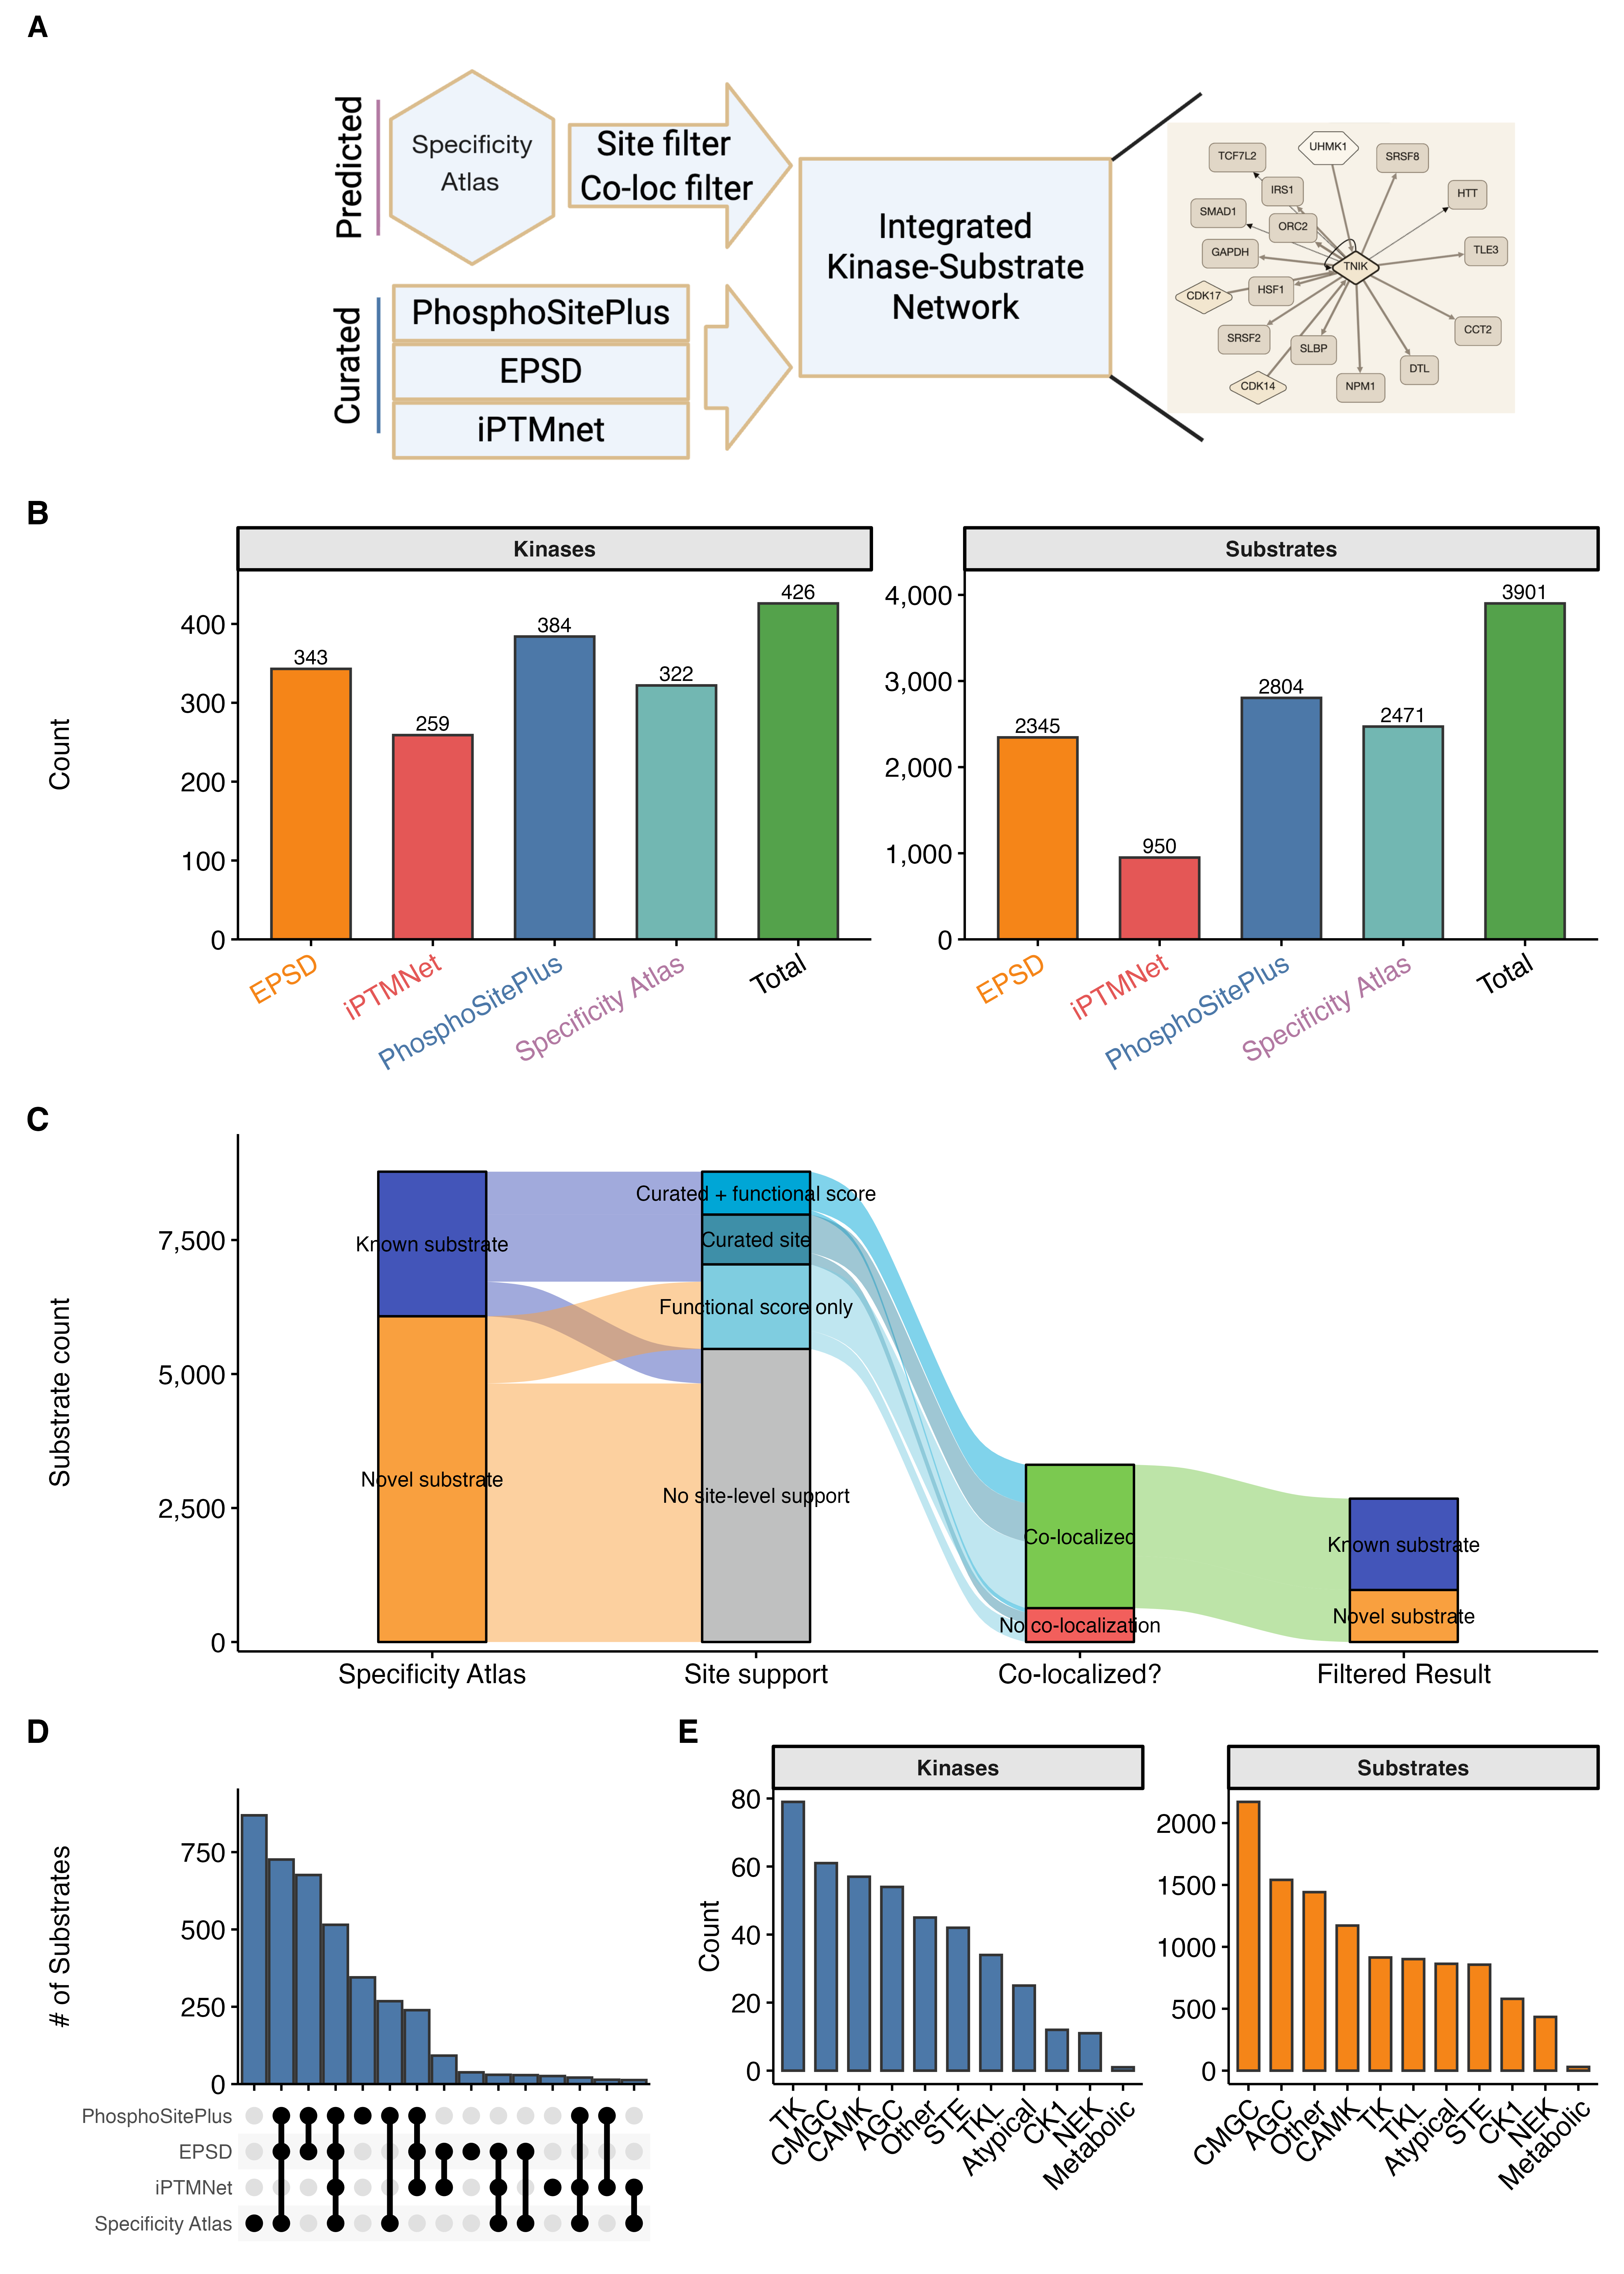
\includegraphics[keepaspectratio]{../figures/paper_figures/fig1.png}}

}

\caption{\label{fig-1}\textbf{Construction of the integrated
kinase-substrate network.} A) Overview of the integration strategy.
Motif-based predictions from the specificity atlas are filtered by
site-level and co-localization criteria and merged with curated KSIs
from PhosphoSitePlus, EPSD and iPTMnet to generate an integrated
kinase-substrate network. An example FLT3-centred neighbourhood
illustrates how curated (solid lines) and predicted (dashed lines)
interactions are combined. B) Numbers of kinases (left) and substrates
(right) contributed by each source and in the integrated total. C)
Alluvial diagram tracking substrates through successive filters.
Substrates are first classified as known vs.~novel (relative to curated
databases), then by whether the modified site is known vs.~novel,
whether the site is predicted to be functional (Ochoa score \(\ge\) 0.5)
vs.~other/unknown, and finally whether the predicted kinase-substrate
pair is co-localized according to the HPA. D) UpSet plot showing overlap
of substrates across the four main KSI sources, highlighting both unique
and shared substrate sets. E) Distribution of kinases (left) and
substrates (right) across major kinase families in the integrated
network.}

\end{figure}%

Alt text: Workflow diagram showing integration of curated
Kinase-Substrate sets with motif predictions, co-localization filters,
and functional scores.

\section{Materials and Methods}\label{materials-and-methods}

\subsection{Curated kinase-substrate
interactions}\label{curated-kinase-substrate-interactions}

We first assembled a non-redundant reference set of human
kinase-substrate-site relationships (``curated KSIs'') from multiple
databases. Primary sources included PhosphoSitePlus (PSP), the
Eukaryotic Phosphorylation Site Database (EPSD) and iPTMnet, which
catalogue experimentally observed phosphosites and often annotate
upstream kinases based on low-throughput experiments or kinase assays
\citep{Hornbeck2015-dg, Chen2025-bt, Huang2018-bq}.

As a starting point, we downloaded the pre-assembled curated KSI table
from the KiNet web portal, which aggregates KSIs from PhosphoSitePlus,
EPSD and iPTMnet and provides kinase annotations \citep{Sekar2024-nx}.
We then re-processed this table to harmonize identifiers and used
available site-level functional annotations needed for our analyses.
Briefly, we extracted the kinase gene symbol, substrate protein,
phosphosite (modified residue and position), source database and/or
PMID. Gene and protein identifiers were harmonized by mapping to
official HGNC gene symbols and UniProt accessions (current versions as
of January 10, 2026). When multiple isoforms existed, phosphosites were
mapped to the reviewed (Swiss-Prot) sequence based on the human proteome
when possible. Phosphosite notation was standardized to a single-letter
residue code plus position (e.g.~``S123''). Redundant entries arising
from overlap across databases were collapsed, while preserving
provenance information (all contributing databases and PMIDs).

Across PhosphoSitePlus, EPSD, iPTMnet and the specificity atlas we
ultimately obtained 13,516 unique phosphosites, with PhosphoSitePlus
contributing the largest number (9,340 sites) and EPSD and the
specificity atlas each contributing substantial additional coverage
(Supp. Figure~\ref{sfig-1}(A)). The overlap structure of these site
sets, including sites unique to individual resources and those shared
across multiple databases, is summarized in
Supp. Figure~\ref{sfig-1}(B). The resulting curated KSI set serves as a
reference baseline for all subsequent analyses, and coverage of kinases
and substrates contributed by each source is shown in
Figure~\ref{fig-1}(B).

\subsection{Kinome-wide motif-based substrate
predictions}\label{kinome-wide-motif-based-substrate-predictions}

To substantially expand beyond known KSIs, we integrated motif-based
predictions from the human kinome specificity atlases for
serine/threonine and tyrosine kinases. Johnson et al.~used
position-specific scoring matrices derived from peptide library screens
to define optimal substrate motifs for the vast majority of human
serine/threonine kinases and subsequently scored reported human
phosphosites against each kinase-specific motif \citep{Johnson2023-ai}.
These matrix-based approaches have been complemented by more recent
deep-learning architectures for phosphorylation site prediction
\citep{Wang2020-nl}. More recently, Yaron-Barir et al.~generated an
analogous atlas for the human tyrosine kinome
\citep{Yaron-Barir2024-lv}. We and others collectively refer to these
resources as the ``specificity atlas''.

We obtained the per-kinase, per-phosphosite prediction scores from the
supplementary materials. For each phosphosite (UniProt accession +
position), the atlases provide a quantitative score or percentile rank
reflecting how well the local sequence matches the optimal motif for
each kinase \citep{Johnson2023-ai, Yaron-Barir2024-lv}. The complete,
unfiltered specificity dataset---containing motif ranks, percentiles,
and promiscuity indices for over 28 million kinase-substrate-site
combinations---is provided as a supplemental resource
(Supp. Table~\ref{stab-1}). From this prediction matrix, we extracted
high-confidence motif-based KSIs using a percentile threshold. Following
the original studies, we focused on phosphosite-kinase pairs in which
the site ranked within the top 10\% of all phosphosites scored for that
kinase (\(\ge\) 90th percentile)
\citep{Johnson2023-ai, Yaron-Barir2024-lv}. This conservative cutoff
retains sites that are strongly preferred by the kinase's motif and
reduces the inclusion of weak, low-specificity matches.

To further mitigate well-known issues with highly promiscuous kinases
whose motifs match a large fraction of the phosphoproteome (e.g.~CK2),
we utilized the provided ``promiscuity index'' for each scored
substrate, defined as the fraction of all phosphosites assigned to the
top 10\% for a given kinase. Substrates above the median promiscuity
were excluded from the motif-based prediction set, as their broad
specificity reduces the utility of purely motif-driven assignments. The
remaining set of motif-supported KSIs was then passed to contextual
filters described below.

\subsection{Contextual filtering}\label{contextual-filtering}

\subsubsection{Subcellular
co-localization}\label{subcellular-co-localization}

Since kinase activity is constrained by spatiotemporal co-localization
with substrates, we filtered motif-based KSIs based on subcellular
localization. We used the HPA subcellular annotations, which provide
antibody- and imaging-based localization calls for thousands of human
proteins across 30 subcellular structures \citep{Thul2017-cl} (HPA
subcellular location dataset, downloaded 10 January 2026). The mapping
of gene-level subcellular compartmentalization used in this study is
provided as a supplemental table (Supp. Table~\ref{stab-2}). For each
kinase and substrate, we retrieved all reported compartments annotated
at the ``Enhanced'', ``Supported'' or ``Approved'' reliability levels,
excluding ``Uncertain'' calls. For every predicted kinase-substrate
pair, we then computed the intersection of kinase and substrate
localization sets and recorded the number of shared compartments, which
is released as a continuous column rather than only as a binary flag.
Pairs with at least one shared compartment were considered co-localized
and retained; pairs with no compartmental overlap were flagged as
unlikely to occur in vivo and removed from the high-confidence set.
Proteins absent from HPA necessarily have no shared compartment and are
therefore treated as non-co-localized, so missing annotation and genuine
spatial separation are not distinguished by this filter. The
distribution of the fraction of motif-predicted substrates that
co-localize with each kinase is shown in Figure~\ref{fig-2}(A); the
median kinase retains 35.5\% of its predicted substrates after applying
this co-localization filter. We note that HPA localizations are neither
exhaustive nor condition-specific, so some genuine context-dependent
interactions may be lost. However, requiring at least one documented
shared localization substantially increases the plausibility of retained
KSIs.

\subsubsection{Phosphosite functional
score}\label{phosphosite-functional-score}

To prioritize phosphosites with higher likelihood of regulatory impact,
we integrated the phosphosite functional score developed by Ochoa et
al., who re-analysed thousands of phosphoproteomics experiments to build
a reference human phosphoproteome and then trained a machine-learning
model to predict functional relevance based on 59 features, including
evolutionary conservation, structural context, regulation patterns and
network properties \citep{Ochoa2020-og}. The resulting score ranges from
0 to 1, with higher values indicating a greater probability that a site
is functionally important.

We downloaded the pre-computed human phosphosite functional scores and
mapped them to our phosphosite identifiers (provided as
Supp. Table~\ref{stab-3}). For each predicted KSI, we annotated the
substrate site with its functional score and designated a site as
``likely functional'' if its score was \(\ge\) 0.5. This is the
threshold recommended by the authors of the score, who report that at a
0.5 cut-off approximately 10\% of the phosphoproteome is retained while
50\% of true-positive functional sites are recovered, making it a useful
cut-off for initial prioritization \citep{Ochoa2020-og}; comparable
thresholds have been applied in subsequent work
\citep{Yaron-Barir2024-lv}. Because any fixed threshold is arbitrary at
its boundary, we additionally report a sensitivity analysis across the
range 0.3-0.7 and release a continuous confidence score (see below). As
expected, tyrosine sites were markedly enriched for site-level support
compared to serine or threonine sites (40.8\% vs.~13.4\% and 15.4\%,
respectively; Figure~\ref{fig-2}(B)). Here, as in Figure~\ref{fig-2}(B),
a site counts as supported if it is either already curated or carries a
functional score above the cutoff; restricting to functional-score
support alone among sites that carry a score gives 31.6\%, 8.2\% and
8.6\%. The difference between residue classes is highly significant
(\(\chi^2\) = 1848.1, df = 2, \(p < 2 \times 10^{-16}\); n = 5,132
tyrosine, 34,754 serine and 7,844 threonine sites). When stratified by
source database, the proportion of scored sites classified as likely
functional ranges from 47.4\% (PhosphoSitePlus) through 50.1\% (EPSD)
and 62.2\% (iPTMnet) to 79.4\% for the specificity atlas layer
(Figure~\ref{fig-2}(C) and Supp. Figure~\ref{sfig-1}(C)). The last of
these is elevated by construction rather than by discovery: functional
score is one of the inclusion criteria for the atlas-derived layer, so
its sites are selected in part on the quantity being measured. The
comparison is informative for the curated sources, which are not
filtered on this score. Unless otherwise noted, analyses focusing on
functional sites consider only motif-based KSIs whose substrate sites
passed this functional score threshold.

\begin{figure}

\centering{

\pandocbounded{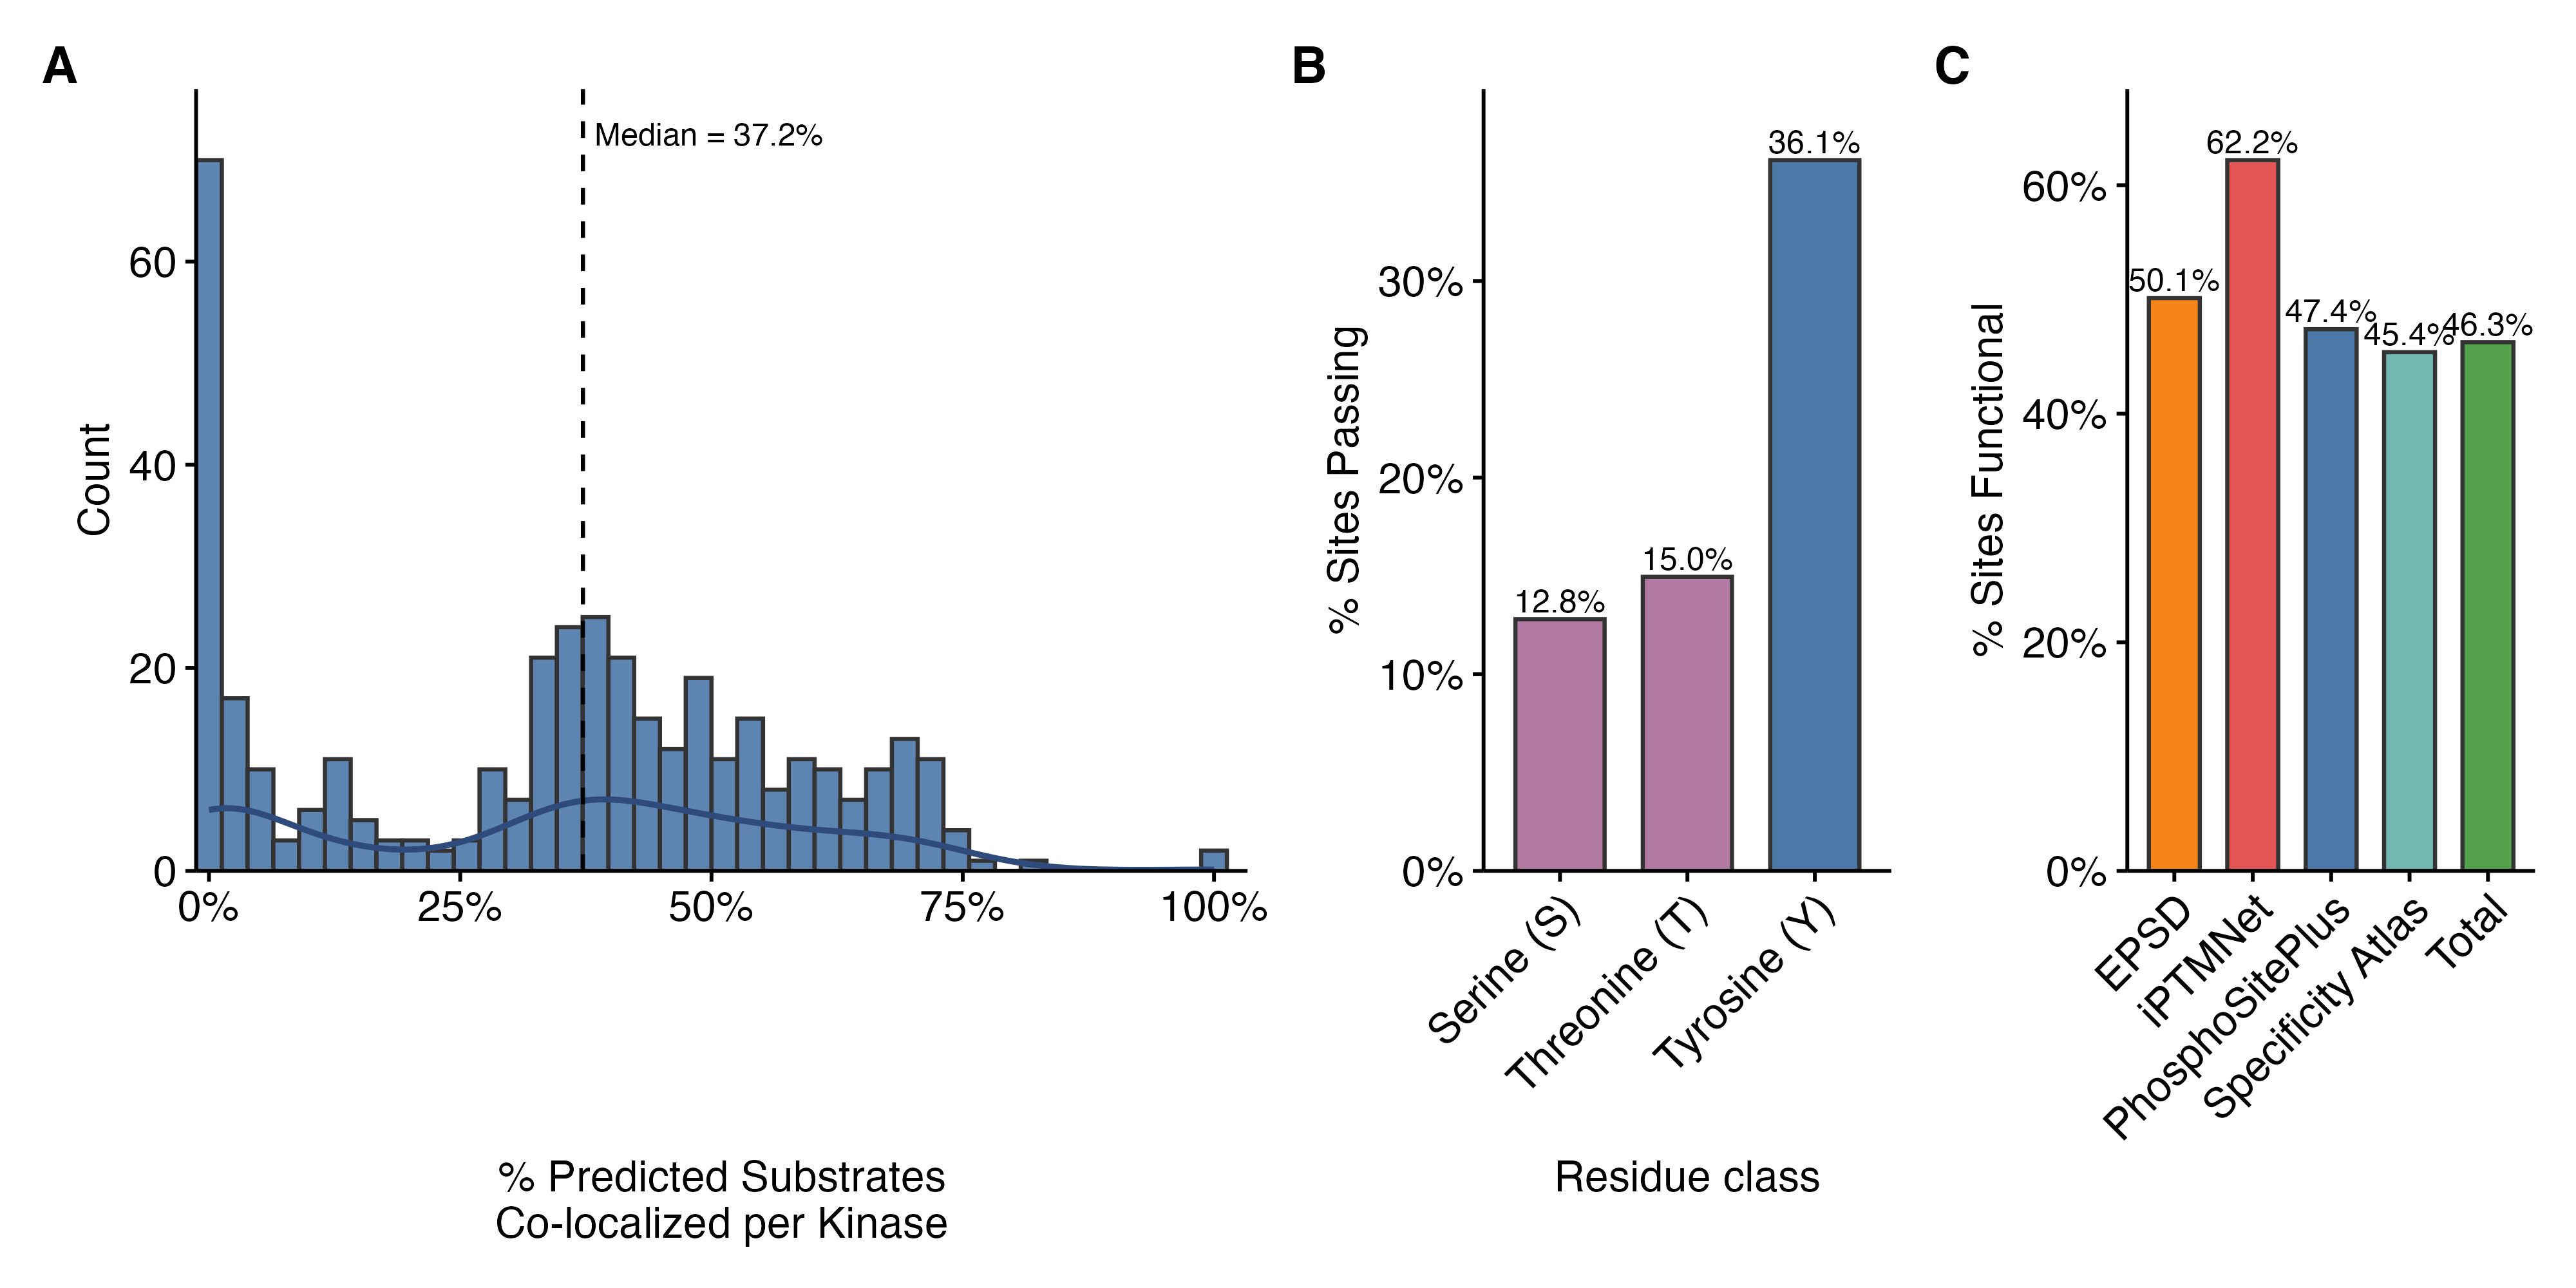
\includegraphics[keepaspectratio]{../figures/paper_figures/fig2.png}}

}

\caption{\label{fig-2}\textbf{Specificity Atlas Filtering Results}. A)
Distribution of subcellular co-localization percentages for predicted
kinase-substrate pairs per kinase. Co-localization was determined using
HPA subcellular location data, requiring at least one shared compartment
between the kinase and substrate. The dashed line indicates the median
co-localization (35.5\%). B) Percentage of predicted sites passing
filtering criteria across residue classes (Serine, Threonine, and
Tyrosine). ``Pass'' is defined as a site being either previously curated
in primary databases (PhosphoSitePlus, EPSD, iPTMNet) or possessing a
high functional score (Ochoa score \(\ge\) 0.5). C) Comparative analysis
of the percentage of functional sites across different data sources,
highlighting the functional density of the predicted atlas relative to
curated repositories.}

\end{figure}%

Alt text: Statistical distribution of phosphosite functional scores
across different residue types (Y, S, T) and source databases.(A) shows
co-localization fraction by kinase;(B) shows functional score enrichment
for tyrosine sites.

\subsection{Integration of motif, localization and
function}\label{integration-of-motif-localization-and-function}

Combining the motif, promiscuity, localization and functional filters,
we defined a high-confidence predicted KSI set as those
kinase-substrate-site triplets that satisfy all of:

\begin{enumerate}
\def\labelenumi{\arabic{enumi}.}
\tightlist
\item
  Motif support: the substrate site ranks in the top 10\% of all
  phosphosites scored for that kinase (\(\ge\) 90th percentile) in the
  relevant serine/threonine or tyrosine atlas.
\item
  Specificity: the site falls below the median promiscuity index,
  excluding sites that are top-ranked for a large fraction of the
  kinome.
\item
  Co-localization: kinase and substrate share at least one HPA-annotated
  subcellular compartment.
\item
  Site-level support: the substrate site either has a phosphosite
  functional score \(\ge\) 0.5 \textbf{or} is already curated in
  PhosphoSitePlus, EPSD or iPTMnet.
\end{enumerate}

Criterion 4 is deliberately a disjunction rather than a conjunction. A
site that has already been curated from the primary literature carries
direct experimental evidence of relevance, so requiring it to
additionally clear a machine-learned functional-score threshold would
discard well-established sites on the basis of a predictor. Curated and
functional-score support are reported as separate columns so that either
can be required independently.

The effect of these filters on the substrate set is visualized as an
alluvial diagram in Figure~\ref{fig-1}(C). This representation tracks
substrates as they transition from known vs.~novel, through known
vs.~novel sites, to likely functional vs.~other sites, and finally to
co-localized vs.~non-co-localized predictions. Although some true
interactions will undoubtedly be excluded (e.g.~transient
co-localization not captured by HPA, functional sites below the
threshold, or kinases with context-dependent specificity), we
deliberately favour specificity over sensitivity to generate a
conservative, high-confidence prediction set. Each predicted KSI is also
cross-referenced to the curated KSI list; interactions present in
curated databases are flagged as ``known'', whereas motif-only
interactions with no curated evidence are classified as novel
predictions contributed by this resource.

\subsection{Species and isoform
handling}\label{species-and-isoform-handling}

The resource is restricted to human proteins (NCBI taxonomy 9606).
Curated interactions were taken from the human subsets of the
contributing databases; non-human entries were not included and no
cross-species orthologue mapping was performed, so a site characterised
only in mouse or rat does not enter the resource on the basis of its
human orthologue. All phosphosite positions are reported against the
canonical (Swiss-Prot) UniProt sequence for the substrate accession.
Where a source record used isoform-specific numbering, the position was
remapped to the canonical sequence, and the UniProt accession is
released alongside every site so that positions can be verified
independently.

\subsection{Substrate and kinase identity
resolution}\label{substrate-and-kinase-identity-resolution}

Resolving protein identity from gene symbols alone is unreliable for
this application, because many legacy protein names are aliases of
several distinct genes. We therefore resolve substrate identity from the
UniProt accession supplied by the specificity atlases, falling back to
the gene symbol only where it maps unambiguously to a single gene.
Kinase identity is resolved from the atlas column names (which use
Manning/CORAL-style short names such as \texttt{P38A}, \texttt{CK1D} and
\texttt{MEK1} rather than HGNC symbols) against a curated kinome
reference table, then against unambiguous aliases, with a small explicit
override list for names that neither source covers; the pipeline halts
if any atlas kinase name remains unresolved rather than silently
discarding it. Every released kinase-substrate-site triplet is checked
automatically against the source atlas to confirm that the site belongs
to the accession it is reported under.

\subsection{Confidence scoring}\label{confidence-scoring}

Alongside the binary criteria above, each predicted interaction carries
a continuous confidence score. Motif percentile and functional score are
each passed through a monotonic, continuously differentiable logistic
transform centred on the corresponding threshold, and localization
evidence is expressed as a saturating function of the number of shared
HPA compartments rather than a binary flag. The composite score is the
unweighted mean of the three components, and all three components are
released as separate columns so that users can reweight or threshold
them independently. This is a transparent re-weighting rather than a
calibrated probability: a fully probabilistic treatment would require
labelled negative examples, which do not exist at kinome scale
\citep{Invergo2022-iv, Horn2014-kx}.

\subsection{Information content of the evidence
layers}\label{information-content-of-the-evidence-layers}

To quantify how much each evidence layer contributes and how far the
layers overlap, we recorded the full joint contingency table of the
three indicators (co-localization, curated-site status and
functional-score support) over all motif-passing kinase-site pairs,
before any of them had been applied. From this table we computed
marginal Shannon entropies, pairwise mutual information, normalised
redundancy (mutual information divided by the smaller of the two
marginal entropies) and conditional mutual information, together with a
leave-one-filter-out analysis quantifying how many pairs each layer
uniquely removes.

\subsection{Annotation of dark
kinases}\label{annotation-of-dark-kinases}

To assess how the integrated network covers dark kinases, we used
DarkKinaseTools and related resources from the NIH Illuminating the
Druggable Genome (IDG) programme to classify kinases as ``understudied
(dark)'' or ``well-studied (light)'' based on publication counts,
functional annotations and available reagents \citep{Berginski2021-so}.
This classification was mapped onto our KSI network, enabling summary
statistics on the proportion of curated vs.~predicted substrates
assigned to dark kinases. We also summarised the fraction of substrates
that are novel (predicted only) for each kinase family
(Figure~\ref{fig-3}(A)) and quantified the fraction of kinase--substrate
pairs involving dark kinases in the curated set versus the
curated-plus-specificity atlas integrated network
(Figure~\ref{fig-3}(B)).

\subsection{Implementation}\label{implementation}

All data integration, filtering and visualisation were performed in R
using the tidyverse ecosystem for data manipulation and plotting. Kinome
annotations and dark/light classifications were obtained via
DarkKinaseTools and associated IDG resources \citep{Berginski2021-so}.
Upset plots showing overlap between resources (for phosphosites and
substrates) were generated using the ggupset package
(Supp. Figure~\ref{sfig-1}(B); Figure~\ref{fig-1}(D)). Scripts used to
download source datasets, perform identifier harmonisation, apply
filters and generate figures are provided in GitHub to facilitate
reproducibility and reuse.

\section{Results}\label{results}

\subsection{Structure and coverage of the integrated
resource}\label{structure-and-coverage-of-the-integrated-resource}

The final resource is organised into two primary tables:

\begin{enumerate}
\def\labelenumi{\arabic{enumi}.}
\tightlist
\item
  \textbf{Kinase-substrate pair table.} This table lists each unique
  kinase--substrate pair (gene symbols), with columns indicating:

  \begin{itemize}
  \tightlist
  \item
    whether the pair is supported by curated databases, motif-based
    predictions, or both;
  \item
    the number, identity and directionality of phosphosites linking the
    kinase and substrate;
  \item
    source databases and PMIDs for curated evidence;
  \item
    motif-related annotations (serine/threonine vs.~tyrosine atlas);
  \item
    contextual evidence flags (co-localization, functional score above
    threshold); and
  \item
    dark/light status of the kinase.
  \end{itemize}
\item
  \textbf{Phosphosite table.} This table lists each unique substrate
  site (UniProt accession, residue, position) together with its assigned
  kinases and annotations, including:

  \begin{itemize}
  \tightlist
  \item
    motif-based scores and ranks for all compatible kinases;
  \item
    flags for high-confidence motif assignments (top 10\%);
  \item
    phosphosite functional score (continuous) and functional
    classification (\(\ge\) 0.5 vs.~\(<\) 0.5);
  \item
    curated vs.~predicted status
  \item
    basic protein metadata.
  \end{itemize}
\end{enumerate}

Across all sources, the integrated resource covers 429 kinases and 3,927
substrate proteins (Figure~\ref{fig-1}(B)). PhosphoSitePlus and EPSD
contribute the largest numbers of substrates, while the specificity
atlas brings in additional substrates not present in curated databases
(Figure~\ref{fig-1}(B)). At the site level, we catalogue 13,516 unique
phosphosites across PhosphoSitePlus, EPSD, iPTMnet and the specificity
atlas (Supp. Figure~\ref{sfig-1}(A)), with substantial but incomplete
overlap between resources (Supp. Figure~\ref{sfig-1}(B)).

In terms of kinase-substrate pairs, the curated KSI set contains 8,364
distinct pairs, while the high-confidence motif-based predictions add
22,613 novel pairs not present in curated databases, for a total of
30,977 distinct pairs (Figure~\ref{fig-3}(C)). Most kinases gain dozens
of novel substrates: the distribution of novel substrates per kinase is
right-skewed, with a median of 46 novel substrates and some kinases
gaining more than 400 (Figure~\ref{fig-3}(D)).

\begin{figure}

\centering{

\pandocbounded{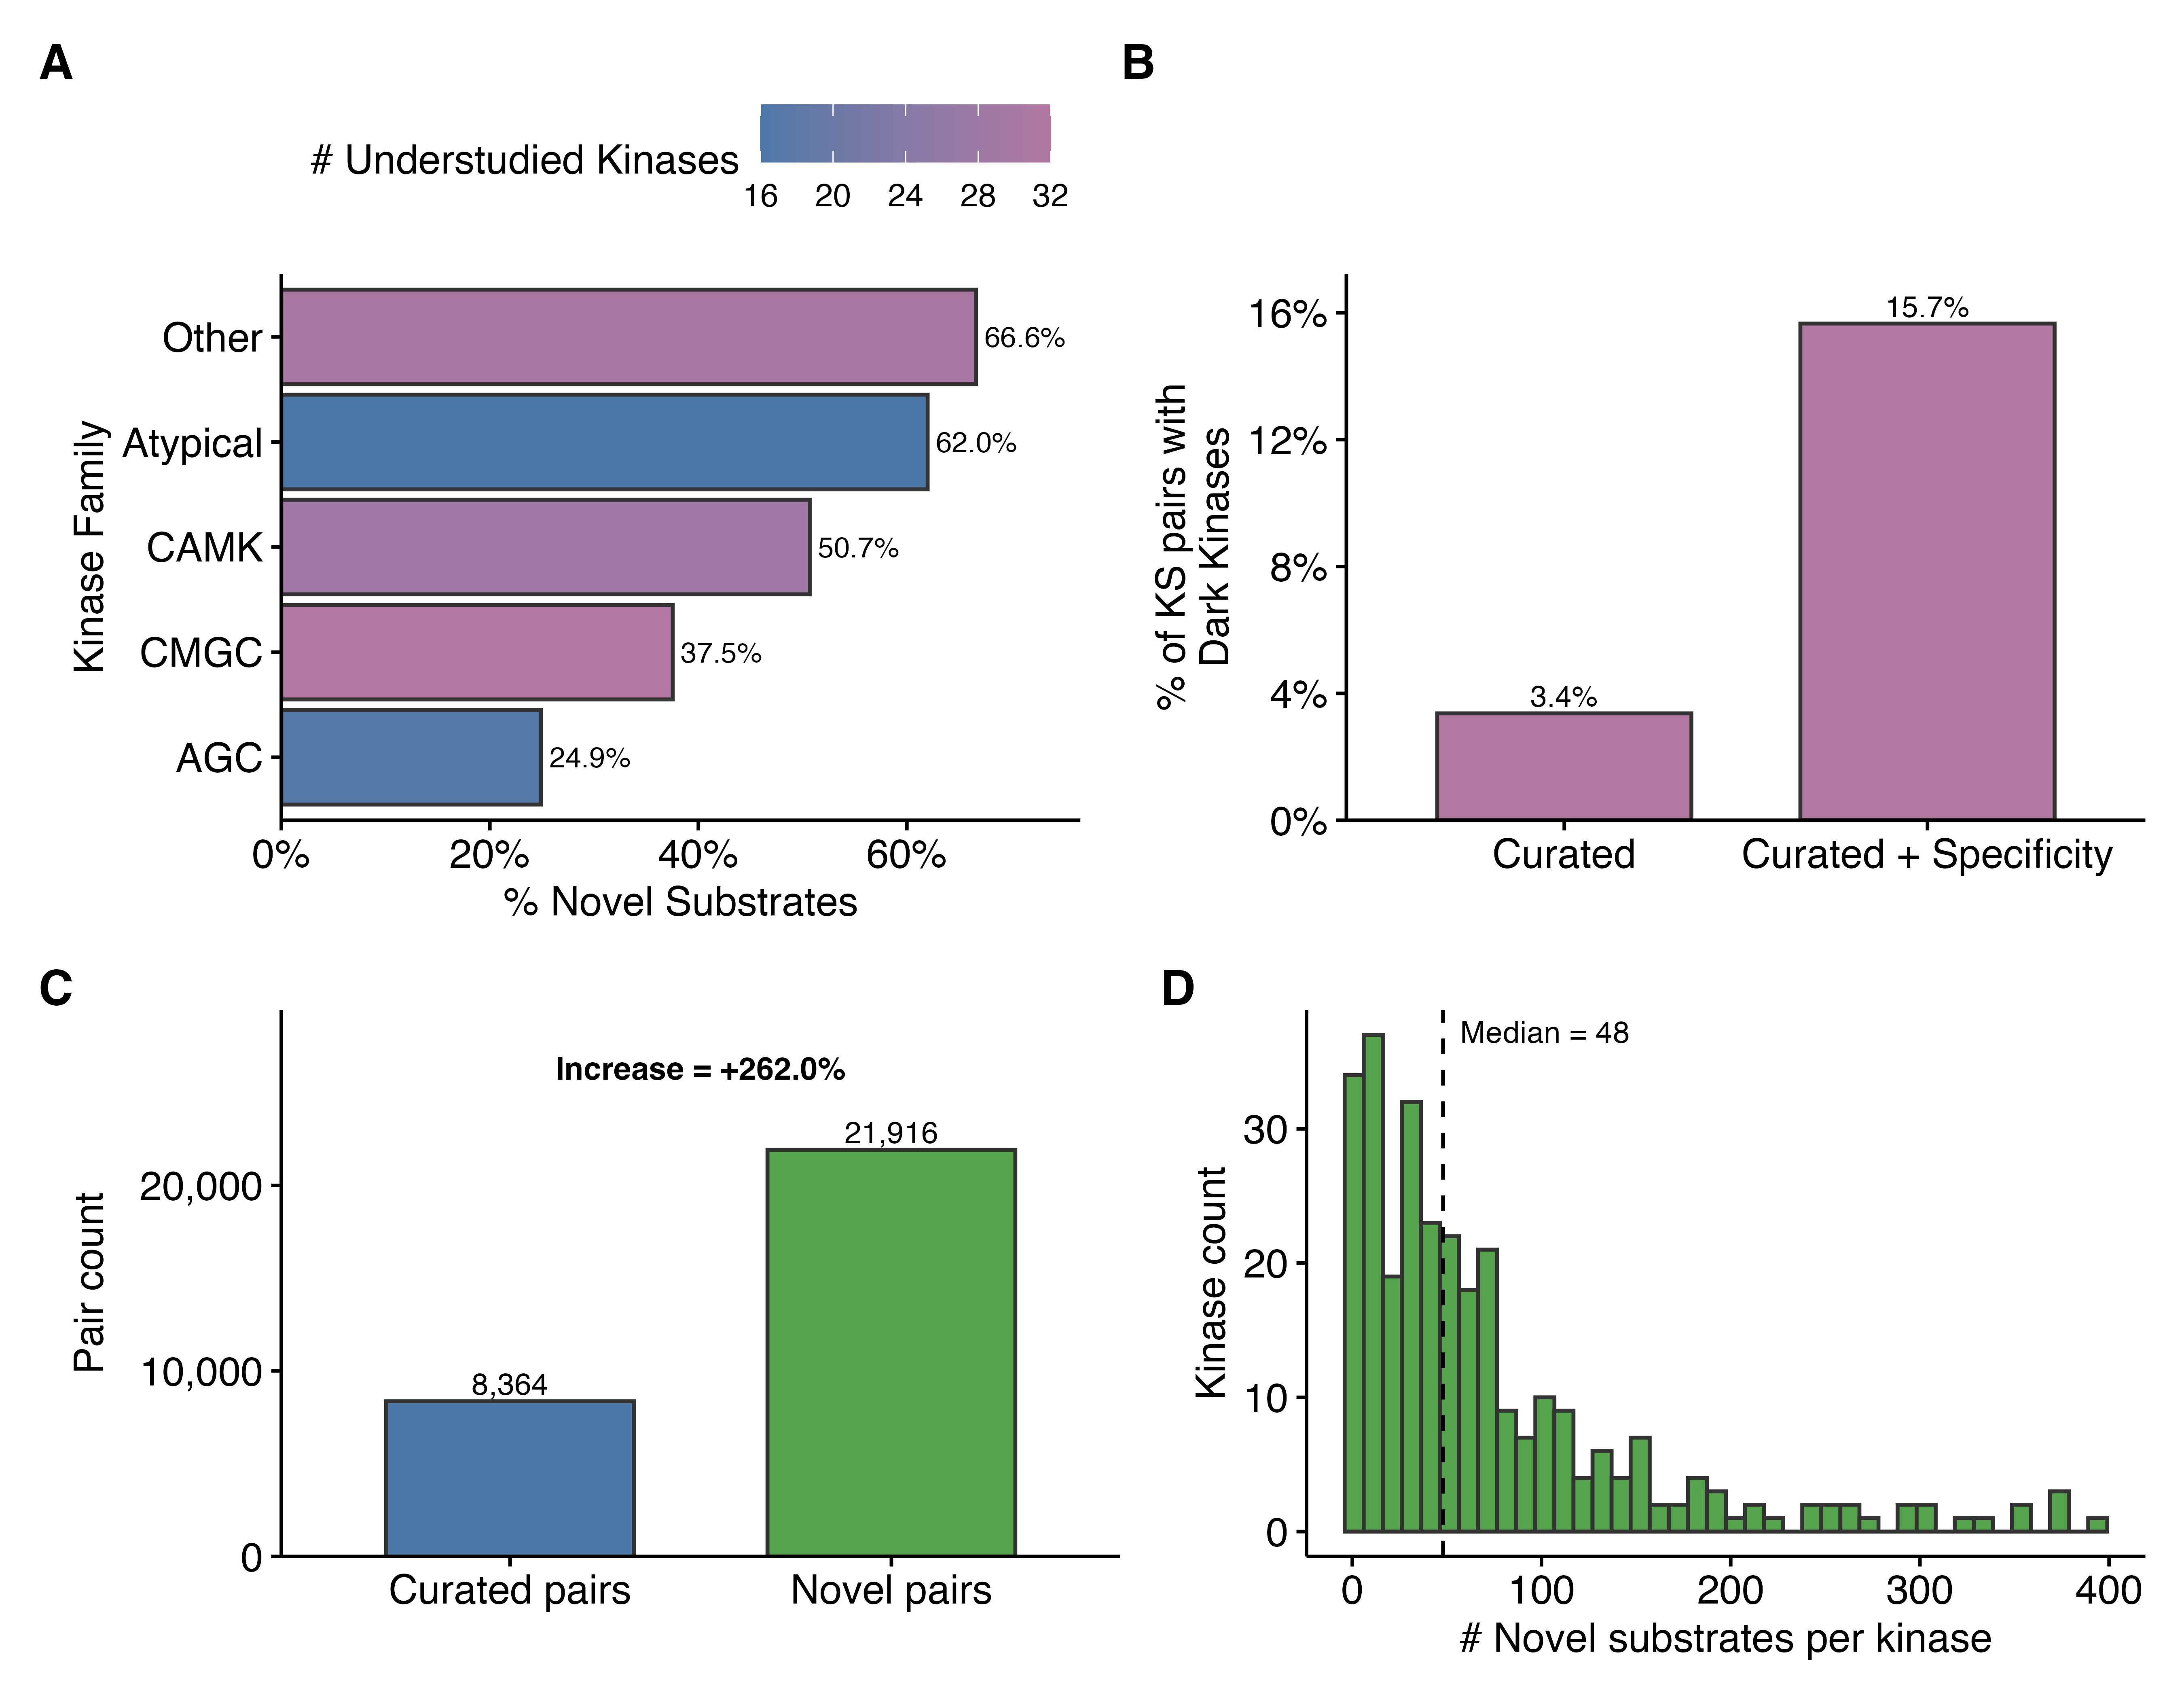
\includegraphics[keepaspectratio]{../figures/paper_figures/fig3.png}}

}

\caption{\label{fig-3}\textbf{Expansion of the known kinase-substrate
network.} A) Fraction of novel substrates across major kinase families.
Bars are colored by the number of dark kinases within each family, as
defined by the IDG (Illuminating the Druggable Genome) classification.
B) Impact of the specificity atlas on the representation of dark
kinases. The bar plot shows the percentage of KS pairs involving
``Dark'' kinases in curated databases versus the combined ``Curated +
specificity atlas'' dataset, demonstrating a significant increase in the
inclusion of dark signaling components. C) Global expansion of the
kinase-substrate (KS) network. The bar plot compares the total number of
curated pairs against novel pairs introduced by the specificity atlas,
showing a roughly four-fold increase in network coverage. D) Histogram
showing the distribution of novel substrates per kinase for kinases
overlapping between curated sources and the specificity atlas. The
dashed line indicates a median of 46 novel substrates per kinase.}

\end{figure}%

Alt text: Comparison of kinase coverage and substrate counts between
curated databases and the integrated resource. Shows a roughly four-fold
increase in KSI pairs and highlights expansion for dark kinases across
different families.

\subsection{Functional and family-level
properties}\label{functional-and-family-level-properties}

Application of the phosphosite functional score retains a large fraction
of sites as likely functional, particularly for tyrosine residues and
for sites drawn from iPTMnet (Figure~\ref{fig-2}(B) and
Supp. Figure~\ref{sfig-1}(C)). After combining motif, co-localization,
and functional filters, the majority of retained substrates pass through
all steps of the pipeline in Figure~\ref{fig-1}(C), indicating that
high-confidence predictions are not dominated by poorly annotated sites
or by non-co-localized pairs.

Kinase and substrate coverage varies across kinase families
(Figure~\ref{fig-1}(E)). TK and CMGC kinases are most numerous, whereas
AGC, CAMK and ``other'' families contribute comparable numbers of
kinases but differ in substrate counts (Figure~\ref{fig-1}(E)). When
focusing on novel substrates, dark kinase families show particularly
high fractions of predicted-only substrates: ``other'' and atypical
kinases have 66.5\% and 61.0\% of their substrates classified as novel,
respectively, while CMGC and CAMK kinases each have \textasciitilde47\%
novel substrates (Figure~\ref{fig-3}(A)). Incorporating the specificity
atlas increases the fraction of kinase--substrate pairs involving dark
kinases roughly five-fold, from 3.3\% in curated databases alone to
16.9\% in the integrated network (Figure~\ref{fig-3}(B)), underscoring
the value of motif-based predictions for illuminating poorly studied
regions of the kinome.

\subsection{Interactive exploration and
visualization}\label{interactive-exploration-and-visualization}

To make these integrated data accessible to the broader community, we
developed KinaseCanvas Explorer, an interactive web application that
enables users to query, filter, and visualize the kinase-substrate
network. The explorer provides a unified interface where users can seed
the graph with a kinase or substrate of interest to generate a local
interaction neighbourhood (see interface in Figure~\ref{fig-4}(A) and
representative output in Figure~\ref{fig-4}(B)). Key features include:

\begin{itemize}
\tightlist
\item
  \textbf{Dynamic Filtering:} Users can toggle between viewing all
  interactions or restricting the view to curated pairs only.
  Additionally, a ``Functional sites only'' filter allows users to focus
  on high-confidence edges supported by phosphosite functional scores.
\item
  \textbf{Visual Distinctions:} Edges are visually encoded to
  distinguish between curated (known) and predicted (novel)
  interactions, as well as between likely functional and other sites.
\item
  \textbf{Graph Layouts:} Multiple layout algorithms (e.g., fCoSE,
  Concentric) are available to optimize the visualization of dense
  networks.
\item
  \textbf{Export Options:} High-quality network images can be exported
  as PNG or PDF files for publication, and the underlying edge data can
  be downloaded as CSV files for further analysis.
\item
  \textbf{Link-outs:} Nodes are linked directly to UniProt, facilitating
  rapid access to detailed protein information.
\end{itemize}

\begin{figure}

\centering{

\pandocbounded{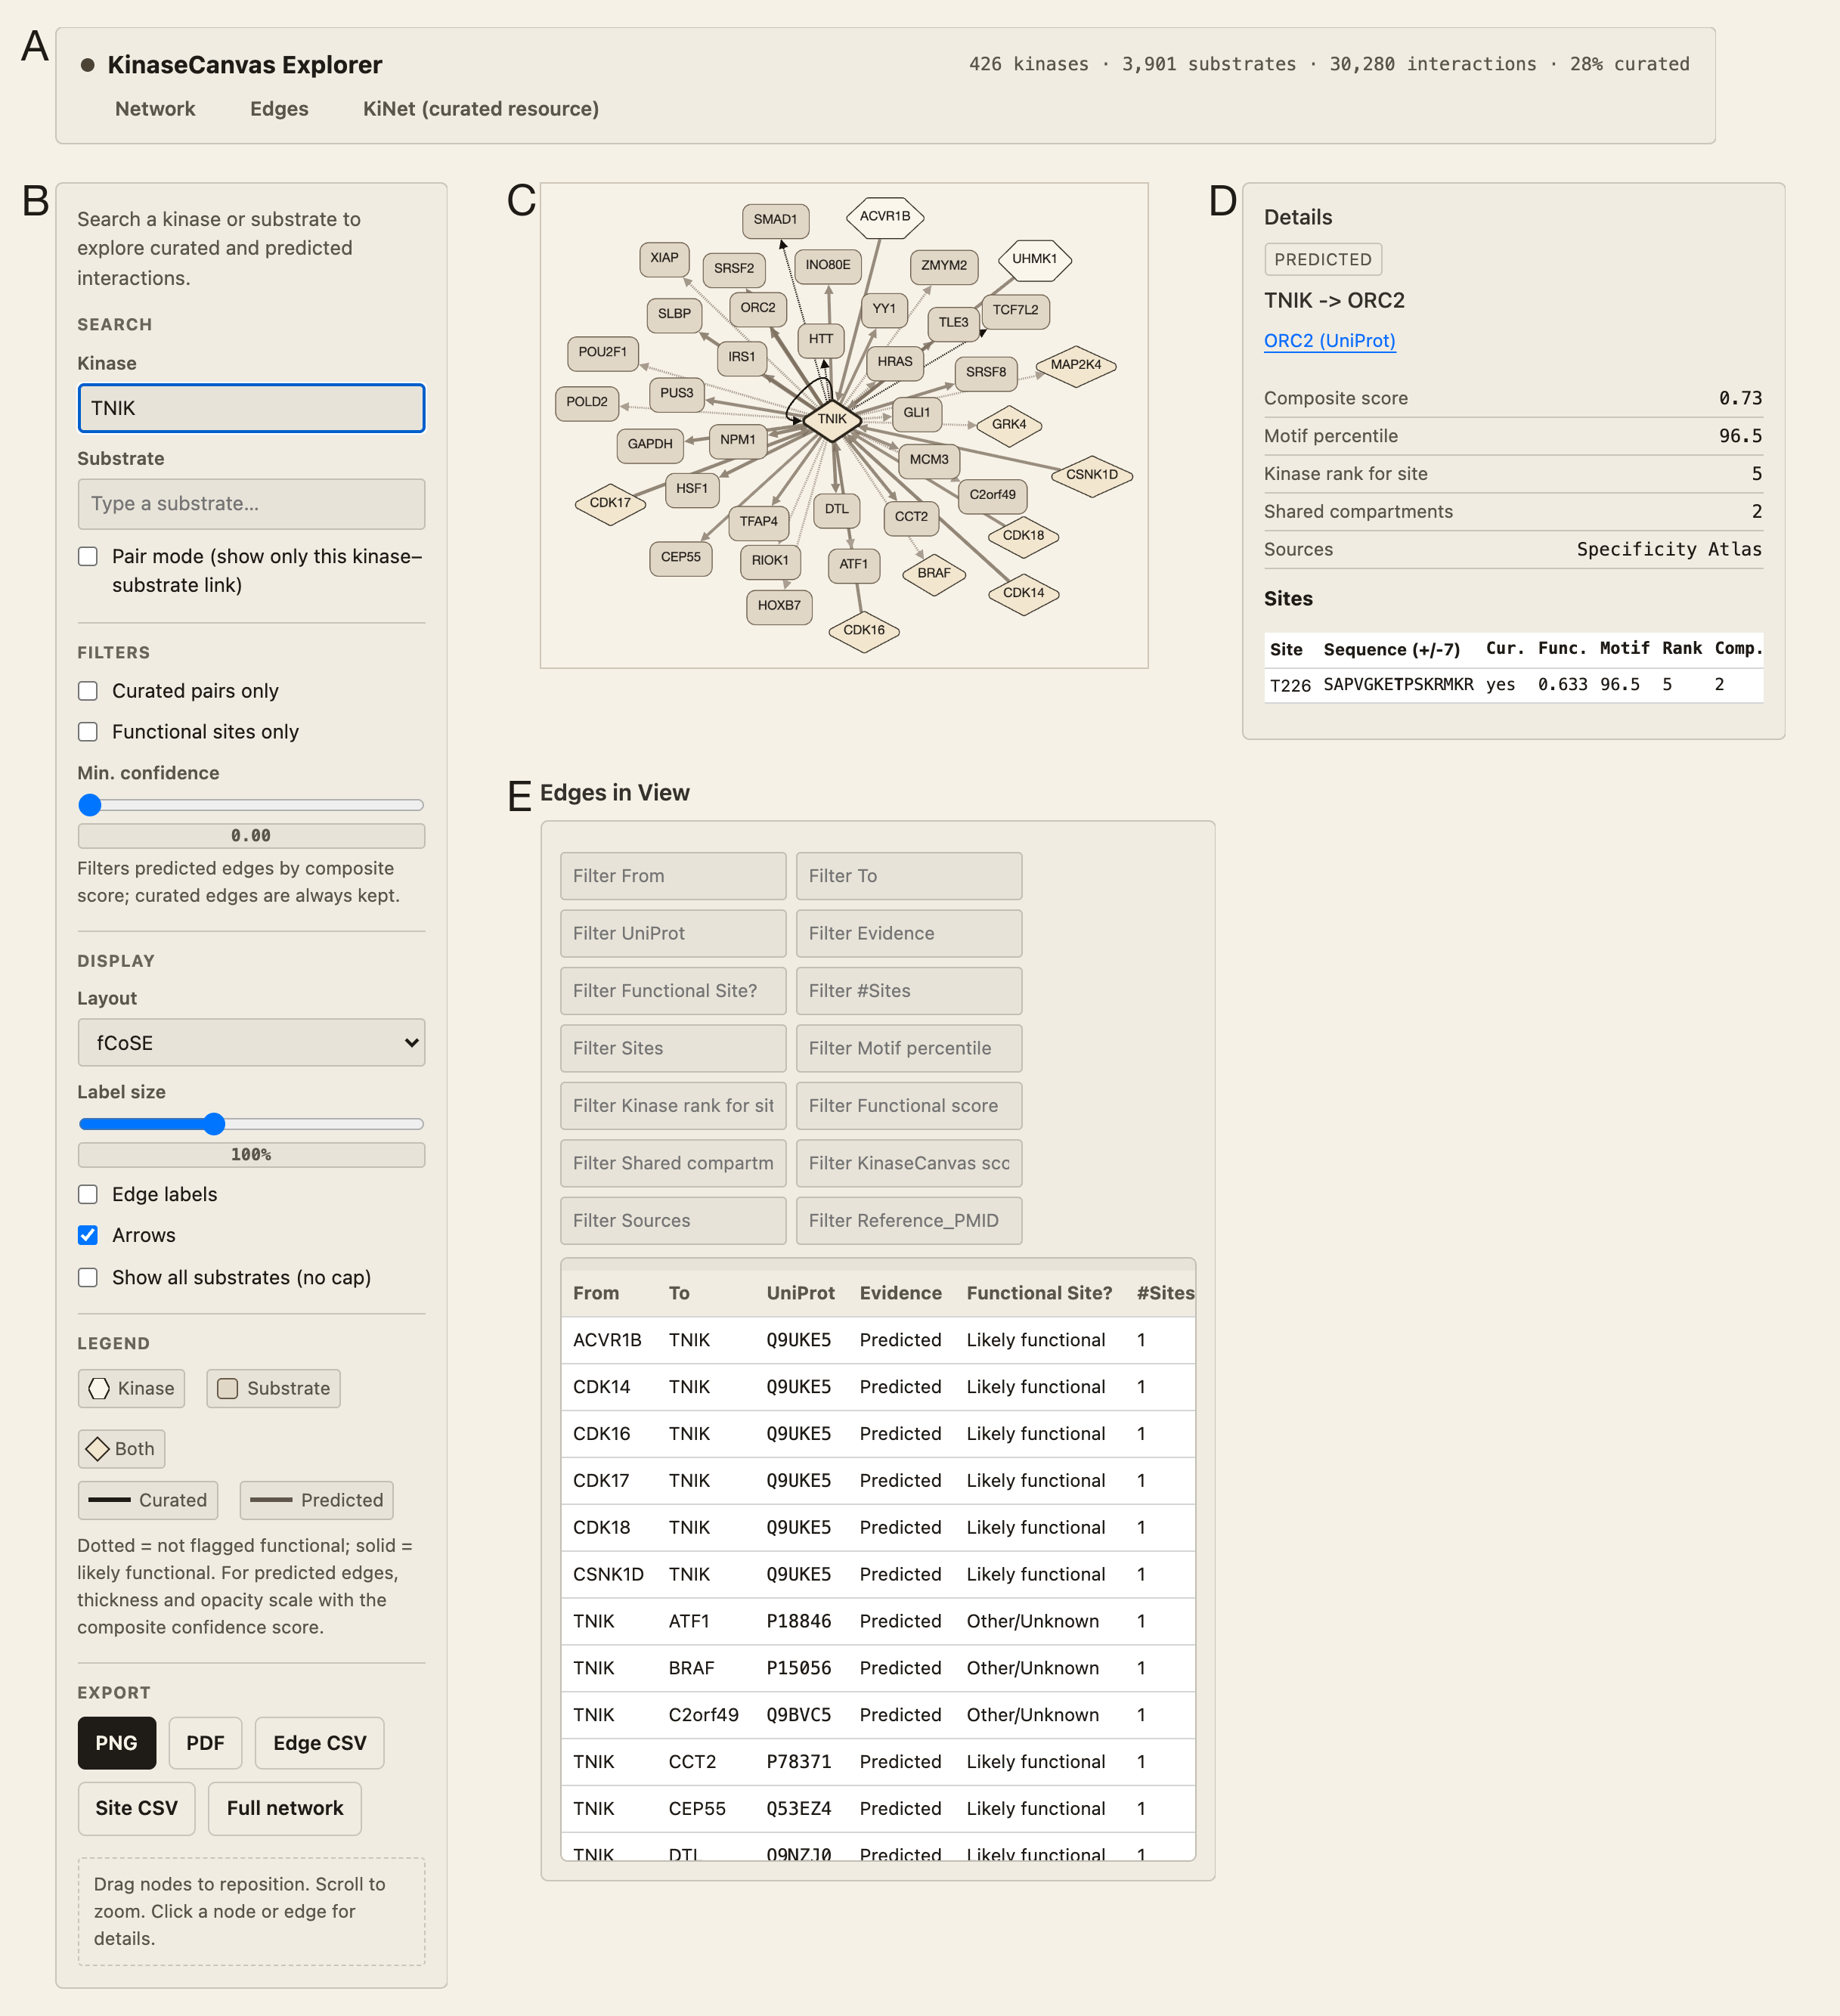
\includegraphics[keepaspectratio]{../figures/paper_figures/fig4.png}}

}

\caption{\label{fig-4}\textbf{Overview of the Kinase-Substrate Resource
Explorer.} A) Banner with summary statistics and preliminary
instructions for explorer use B) Sample graph using the kinase TNIK
(TRAF2 and NCK interacting kinase) as a representative seed. The central
viewport displays an interactive graph of known and predicted
substrates. Edges are styled to differentiate between curated (dark
colored) and predicted (light colored) interactions, with solid lines
indicating likely functional sites and dotted lines representing
interactions of unknown functional impact}

\end{figure}%

Alt text: Interactive explorer interface displaying kinase-substrate
interaction network graph with legend differentiating curated (dark
colored) versus predicted (light colored) interactions and functional
significance of phosphosites.

By combining intuitive visualization with robust filtering, the
KinaseCanvas Explorer empowers researchers to rapidly generate
hypotheses about kinase function and substrate regulation in a
context-aware manner.

\section{Discussion}\label{discussion}

We have developed a comprehensive resource that combines
literature-curated phosphorylation data with empirically measured,
kinome-wide substrate specificity profiles to chart the human
kinase--substrate network. This addresses a major gap in cell-signalling
knowledge: despite decades of study, substrates are still unknown or
poorly defined for most human kinases
\citep{Dinkel2011-pp, Hu2014-dp, Berginski2021-so}. By leveraging recent
motif profiles for \textasciitilde90\% of the human kinome
\citep{Johnson2023-ai, Yaron-Barir2024-lv}, we systematically expand
substrate lists for hundreds of kinases and then constrain these
predictions with biologically motivated filters for co-localization and
phosphosite functionality. The result is a collection of KSI hypotheses
that is both broad---increasing the number of candidate KSIs roughly
four-fold relative to curated databases alone
(Figure~\ref{fig-3}(C))---and enriched for plausible, potentially
regulatory interactions (Figure~\ref{fig-1}(A); Figure~\ref{fig-2}(A);
Supp. Figure~\ref{sfig-1}(A)).

\subsection{Relationship to existing
resources}\label{relationship-to-existing-resources}

Traditional resources such as PhosphoSitePlus, EPSD and iPTMnet grow as
new experimental data and curated literature are added
\citep{Hornbeck2015-dg, Chen2025-bt, Huang2018-bq}. These databases
provide high-confidence KSIs, but their coverage is limited by
experimental throughput and publication bias towards a small set of
kinases and pathways \citep{Berginski2021-so}. The recently introduced
KiNet web portal builds directly on these curated datasets by
aggregating interactions from PhosphoSitePlus, EPSD and iPTMnet,
annotating kinases with group membership and pathway/domain context, and
providing interactive network visualisations for user-selected protein
sets \citep{Sekar2024-nx}.

Our work is complementary to, and explicitly builds on, KiNet. We use
the KiNet-integrated KSI network as the starting curated set, but then
extend it in three major ways. First, we overlay kinome-wide,
empirically measured substrate specificity atlases for serine/threonine
and tyrosine kinases \citep{Johnson2023-ai, Yaron-Barir2024-lv} to infer
motif-supported kinase--phosphosite edges that are not yet observed
experimentally (Figure~\ref{fig-3}(C)). Second, we integrate orthogonal
contextual information: subcellular localization from HPA
\citep{Thul2017-cl} and phosphosite functional scores from Ochoa et al.
\citep{Ochoa2020-og} to filter and prioritize predicted interactions
(Figure~\ref{fig-1}(A); Figure~\ref{fig-2}(A);
Supp. Figure~\ref{sfig-1}(A)). Third, we systematically quantify how
these additions expand coverage for dark kinases and for different
kinase families (Figure~\ref{fig-3} (A, B)). In practical terms, whereas
KiNet focuses on exploring known KSIs across pathways and protein sets,
our resource aims to ``fill in'' missing edges by providing a ranked,
context-aware set of candidate interactions centred on phosphosite-level
properties.

The Kinase Library web portal \citep{Johnson2023-ai} serves as the
primary interface for the Johnson et al.~and Yaron-Barir et al.~atlases,
allowing users to score specific peptide sequences against kinase
motifs. However, it is designed for sequence-level queries rather than
network exploration. Similarly, tools like the KSEA App enable
kinase-substrate enrichment analysis but often rely on curated databases
or require users to upload custom specificity matrices, and do not
provide a browsable network of high-confidence predictions.

Earlier motif-based tools such as NetPhorest, Scansite and GPS used
consensus sequence motifs and position-specific scoring matrices
compiled from smaller sets of peptide library experiments or
literature-derived substrates
\citep{Miller2008-ey, Obenauer2003-fc, Wang2020-hj}. These resources
proved useful for hypothesis generation but were limited in kinase
coverage and often relied on consensus motifs shared across related
kinases. The specificity atlases used here are broader in scope,
profiling hundreds of human kinases with oriented peptide libraries and
scoring essentially the entire known human phosphoproteome
\citep{Johnson2023-ai, Yaron-Barir2024-lv}. By intersecting these
empirically derived motif scores with orthogonal features we
substantially improve the signal-to-noise ratio relative to motif scores
alone. This multi-layer integration is aligned with a broader trend in
systems biology toward combining complementary datasets and prior
knowledge to infer more accurate signalling networks
\citep{Ochoa2020-og, Yaron-Barir2024-lv, Licata2020-fm}.

\subsection{Motif models derived from peptide libraries and from in
vitro
phosphoproteomics}\label{motif-models-derived-from-peptide-libraries-and-from-in-vitro-phosphoproteomics}

The motif layer of this resource is built on positional-scanning peptide
library data \citep{Johnson2023-ai, Yaron-Barir2024-lv}, and it is worth
being explicit about what that choice does and does not buy. Peptide
libraries measure the intrinsic preference of the catalytic cleft
against a degenerate synthetic background, which gives uniform coverage
across the kinome but can have modest signal-to-noise for individual
kinases and, by construction, reports only what the active site sees. An
orthogonal strategy is to phosphorylate dephosphorylated proteome
extracts with individual recombinant kinases and read out the products
by mass spectrometry, as done by Sugiyama et al.~for 385 kinases
\citep{Sugiyama2019-ki}. That design presents kinases with real protein
substrates in native sequence context, and several groups have since
converted the resulting data into position-specific matrices suitable
for scoring: Poll et al.~derived position-dependent Shannon information
matrices for 384 kinases \citep{Poll2024-km}, and Invergo built
position-specific scoring matrices and naive Bayes classifiers from the
same source \citep{Invergo2022-iv}.

These two experimental designs are complementary rather than competing.
Poll et al.~compared their mass-spectrometry-derived logos directly
against the peptide-library motifs used here and reported a high degree
of concordance, concluding that the best predictions are likely to come
from combining both data types \citep{Poll2024-km}. We regard a
systematic head-to-head comparison of peptide-library and in vitro
phosphoproteomic specificity models -- matched for kinase coverage and
evaluated against a common set of curated interactions -- as an
important next study, and one that would be better served by a dedicated
benchmarking paper than by a resource description. In the meantime,
users should understand the motif layer of KinaseCanvas as one
particular, uniformly measured view of intrinsic specificity rather than
as a complete model of substrate recognition.

\subsection{Orthogonality and information content of the evidence
layers}\label{orthogonality-and-information-content-of-the-evidence-layers}

A reasonable concern about any resource that stacks filters is whether
the layers are actually independent, or whether they largely re-encode
the same signal. We addressed this directly by computing the joint
distribution of the three indicators across all motif-passing
kinase-site pairs. Subcellular co-localization carries by far the most
entropy of the three layers (0.91 bits, versus 0.42 bits for
curated-site status and 0.43 bits for functional-score support), simply
because it partitions the candidate set more evenly. More importantly,
the layers are close to orthogonal: pairwise mutual information is
0.0007 bits between co-localization and curated status, 0.0007 bits
between co-localization and functional score, and 0.0082 bits between
curated status and functional score, corresponding to normalised
redundancies of 0.2\%, 0.2\% and 2.0\% respectively. Conditioning on the
third indicator does not change this picture.

It is worth noting where the residual redundancy actually lies. The
functional score of Ochoa et al. is trained on 59 features spanning
mass-spectrometry evidence, phosphosite regulation, structural
environment and evolutionary conservation, and one of those features is
how well a site matches a kinase specificity model \citep{Ochoa2020-og}.
The motif layer and the functional score are therefore expected to share
some information by construction, and the small but largest observed
redundancy -- between curated status and functional score -- is
consistent with both depending on how thoroughly a site has been
observed. Subcellular localization, by contrast, is not among the
features of the functional score, and the measured redundancy confirms
that it contributes essentially independent evidence. In practical terms
the co-localization filter is doing substantial work rather than
rubber-stamping decisions already made: it uniquely removes 46,159
kinase-site pairs that pass the site-level criteria, and omitting it
would inflate the high-confidence set by 173\%.

\subsection{Biological insights from the integrated
network}\label{biological-insights-from-the-integrated-network}

The integrated network reveals several notable features of
kinase-substrate annotation. First, the distribution of novel substrates
across kinases is highly non-uniform (Figure~\ref{fig-3}(D)). Many
kinases with already rich substrate annotations gain additional
predicted substrates but do not dominate the novel interaction set,
partly because of our promiscuity and functional filters. In contrast, a
large number of kinases with few or no curated substrates acquire dozens
of predicted substrates, often with strong motif support, high
phosphosite functional scores and clear co-localization with substrates
(Figure~\ref{fig-1}(A); Figure~\ref{fig-2}(A); Figure~\ref{fig-3}(C)).
This pattern is particularly evident among dark kinases, for which more
than half of substrates are novel predictions in several kinase families
(Figure~\ref{fig-3}(A)). The fraction of KSI pairs involving dark
kinases increases from 3.3\% in curated databases alone to 16.9\% in the
integrated network (Figure~\ref{fig-3}(B)), highlighting the potential
of motif-informed approaches to illuminate poorly characterised parts of
the kinome \citep{Berginski2021-so}.

Second, our residue-level analyses show that tyrosine sites are both
less frequent and more strongly enriched for site-level support than
serine or threonine sites: 40.8\% of tyrosine sites in our resource are
either already curated or carry a functional score above the threshold,
compared with 13.4\% of serine and 15.4\% of threonine sites
(Figure~\ref{fig-2}(B)); the corresponding functional-score-only
figures, among sites carrying a score, are 31.6\%, 8.2\% and 8.6\%. We
report this as a property of the assembled resource rather than as a
claim about the phosphoproteome, because several factors plausibly
contribute to it and we cannot separate them here. Much of the available
phosphotyrosine data was generated using anti-phosphotyrosine
immunoaffinity enrichment \citep{Rush2005-py}, a targeted design that
both concentrates on sites of prior biological interest and differs
systematically from the untargeted enrichment used for serine and
threonine sites. Phosphotyrosine is also the smallest and best-studied
of the three classes, so its coverage is comparatively closer to
saturation, and a substantial share of well-characterised tyrosine sites
are receptor tyrosine kinase autophosphorylation sites whose documented
function is to recruit SH2- and PTB-domain effectors
\citep{Miller2018-hi}. Any of these would raise the apparent
functional-score enrichment of tyrosine sites independently of
underlying regulatory importance. Published analyses likewise report
that tyrosine and serine/threonine phosphorylation differ in their
regulatory character and in the depth to which each has been sampled
\citep{Sharma2014-ud, Ochoa2020-og}, and the relative evolutionary
conservation of phosphothreonine and phosphotyrosine sites remains an
area of active disagreement \citep{Landry2009-wf, Ochoa2020-og}. We
therefore draw no evolutionary inference from this observation.

Such functional enrichment is exemplified by our prediction of the ABL1
kinase phosphorylating the ARID1A tumor suppressor at Y762. While this
phosphosite is currently absent from major curated databases like
PhosphoSitePlus, it appears as a high-confidence candidate for ABL1
(ranked 2nd, 96th percentile) in the tyrosine specificity atlas
\citep{Yaron-Barir2024-lv}. The site possesses an Ochoa functional score
\(\ge\) 0.5, and both the kinase and substrate are verified to
co-localize in the nucleoplasm. Given ABL1's established role as a major
oncogenic driver \citep{Druker2001-fn} and ARID1A's status as a critical
subunit of the SWI/SNF chromatin-remodeling complex frequently mutated
in ovarian and gastric cancers \citep{Wiegand2010-di, Wang2011-vb}, this
motif-supported link suggests a potential regulatory axis that has
remained overlooked in current curated networks.

Similarly, our resource illuminates potential regulatory roles for dark
kinases. For example, the NEK6 kinase, despite its known role in mitotic
spindle formation and its frequent overexpression in human tumors
\citep{Gao2025-pt}, remains relatively under-annotated at the substrate
level. Our pipeline identifies KIFAP3 (kinesin-associated protein 3), a
subunit of the kinesin-2 motor complex essential for intracellular
transport and ciliogenesis \citep{Onodera2021-eh}, as a high-confidence
substrate for NEK6. Specifically, we predict NEK6 phosphorylation of
KIFAP3 at S25 as a novel, likely functional site supported by shared
localization in the nucleoplasm and cytosol. This predicted interaction
suggests a mechanism by which NEK6 may coordinate cell-cycle progression
with microtubule-based transport, providing a prioritized candidate for
downstream experimental validation.

Third, the family-wise patterns in Figure~\ref{fig-1}(E) and
Figure~\ref{fig-3}(A) imply that certain kinase groups such as atypical
and ``other'' kinases may be systematically under-annotated at the
substrate level. For these groups, more than half of substrates in our
resource are novel, motif-supported predictions (Figure~\ref{fig-3}(A)).
This suggests that a substantial fraction of phosphorylation events
currently attributed to generic ``proline-directed'' or ``acidic''
kinases could, in fact, be mediated by less-characterised kinases with
similar motifs but distinct biological roles. Experimental testing of
these candidates using targeted kinase perturbation combined with
phosphoproteomics or substrate-trapping mutants could reveal new
pathways and cross-talk among kinase families
\citep{Miller2008-ey, Linding2007-rk, Gerritsen2021-cr, Liu2023-re}.

\subsection{Limitations and caveats}\label{limitations-and-caveats}

Despite the stringent filtering, our predictions remain hypotheses and
not confirmed in vivo interactions. Several limitations merit
consideration. First, kinases with highly similar motifs (e.g., AKT
vs.~SGK, or different MAPKs) will often share predicted substrates
\citep{Johnson2023-ai, Miller2018-hi, Muller-Dott2025-yf}.
Sequence-based motif scoring alone cannot always discriminate which
kinase is responsible for a given phosphosite in a particular cell type
or condition. Our co-localization filter removes obvious mismatches
(e.g., a mostly cytosolic kinase and an exclusively nuclear substrate),
but does not capture dynamic relocalization, scaffold-mediated proximity
or compartment-specific isoforms. As a consequence, some true
interactions may be excluded, while some retained interactions may occur
only in specific contexts not captured by current localization data
\citep{Thul2017-cl}. Users should therefore treat the predicted kinase
list for each phosphosite as a set of candidates to be prioritised
rather than a definitive assignment.

Second, we consider each phosphosite largely in isolation, whereas
substrate recognition in vivo depends on determinants that lie outside
the +/-7 residue window a position-specific matrix can see
\citep{Miller2018-hi}. Kinases are recruited to substrates through
docking interactions distinct from the catalytic cleft, including the D-
and DEF-motifs used by MAP kinases and the SH2- and PTB-domain
interactions that bring receptor tyrosine kinase substrates to high
effective local concentration \citep{Miller2018-hi}. A peptide that
scores poorly against a kinase's linear motif can therefore still be an
efficient substrate once bound. Recognition is also frequently
hierarchical: casein kinase 1 requires a phosphorylated residue at n-3,
GSK3 at n+4, and casein kinase 2 can use either canonical or
phospho-determinants, so a site's suitability depends on prior
modification events that a static motif score does not represent
\citep{Miller2018-hi}. A site that matches a kinase motif may equally
remain unphosphorylated if it is buried in the folded protein or if an
upstream priming event is absent. Conversely, kinases can act on
multiple sites within the same substrate, and combinatorial patterns of
phosphorylation may be required for functional output. Our use of a
phosphosite functional score partially accounts for evolutionary
conservation, structural features and regulatory behaviour
\citep{Ochoa2020-og}, but cannot fully model three-dimensional
accessibility or cooperative phosphorylation events. Taken together,
these mechanisms bias a top-percentile motif tier against precisely
those kinases for which docking, rather than the catalytic cleft,
dominates substrate selection -- which is one reason we also release a
continuous confidence score and a relaxed motif tier. Incorporating
structural information, as done in 3D-aware prediction tools, and
explicit modelling of docking and priming determinants would improve
specificity for kinases with overlapping linear motifs
\citep{Miller2018-hi, Liu2023-re}.

Third, every criterion in the pipeline is applied as a threshold, and
thresholds are arbitrary at their boundaries. A site scoring 0.4999 on
the functional score is excluded while one scoring 0.5001 is retained,
and once retained the two are treated identically even though a site
scoring 0.99 is far better supported. We have taken three steps to
mitigate this rather than defend it. The cut-offs themselves are not
arbitrary in origin -- 0.5 is the value the authors of the functional
score recommend for initial prioritization \citep{Ochoa2020-og} and the
90th motif percentile follows the specificity atlases
\citep{Johnson2023-ai, Yaron-Barir2024-lv}. We report a sensitivity
analysis across functional-score cut-offs from 0.3 to 0.7 and motif
percentiles from the 80th to the 99th, so readers can see which
conclusions depend on the operating point and which do not. And every
released interaction now carries a continuous confidence score built
from smooth, monotonic transforms of the underlying quantities, so users
who prefer ranking to filtering are not forced into our binary
decisions. A fully probabilistic treatment -- in which each evidence
layer contributes a calibrated likelihood and predictions carry
posterior probabilities -- would be preferable still, but it requires
labelled negative examples that do not exist at kinome scale; approaches
of this kind have so far been built either on curated positives with
sampled decoys or on in vitro assay data
\citep{Invergo2022-iv, Horn2014-kx}, and extending them across the whole
kinome is a substantial methods problem in its own right.

Fourth, our filters are spatial but not temporal. Requiring a kinase and
substrate to share a subcellular compartment is a necessary condition
for a genuine interaction, not a sufficient one: a real kinase-substrate
pair should additionally show coordinated behaviour over time, with
substrate phosphorylation tracking kinase activity across stimuli,
inhibitor treatments or genetic perturbation. Compendia of perturbation
phosphoproteomics now make this tractable in principle
\citep{Ochoa2016-kr, Muller-Dott2025-yf}, and adding a co-regulation
layer -- either as an additional evidence component or as a filter in
its own right -- is the most obvious way to sharpen the resource beyond
what static annotation can achieve.

Fifth, while our filters substantially reduce the apparent
false-positive rate, they may also disproportionately remove
interactions in less-characterised cellular compartments or tissues,
where localization and functional annotations are sparse. For example,
proteins restricted to specific organelles or cell types may lack
high-confidence HPA annotations, causing their interactions to be
under-represented (Figure~\ref{fig-2}(A)). Future expansions of
localization resources and condition-specific phosphoproteomics will be
important to mitigate this bias \citep{Thul2017-cl, Uhlen2015-sd}.

Finally, we focus on the presence of potential kinase-substrate
relationships rather than their quantitative strength or regulatory sign
(activating vs.~inhibitory). Integrating quantitative phosphoproteomic
time series with prior KSI networks has been shown to enable inference
of causal directionality and sign \citep{Invergo2020-kl}. Extending our
resource with such information is a promising direction but beyond the
scope of the current study.

\subsection{Future directions}\label{future-directions}

Several extensions could further enhance the resource. First,
incremental updates can incorporate new phosphosites, additional motif
profiling experiments and improved functional annotations. As kinase
specificity profiling is completed for remaining kinases and refined
under different conditions \citep{Johnson2023-ai, Yaron-Barir2024-lv},
our pipeline can be rerun to refresh motif-based predictions and
coverage. Second, dynamic data could be used to refine or reweigh
predicted interactions. Condition-specific phosphoproteomics, kinase
inhibition or knockdown experiments, and proximity-labelling assays can
provide direct evidence for or against particular KSIs
\citep{Ochoa2020-og, Miller2008-ey, Gerritsen2021-cr}. Such data could
be integrated into probabilistic or machine-learning models that jointly
consider motif score, co-localization, co-expression, network proximity
and experimental perturbation response to yield an overall confidence
score, as done in other kinase--substrate prediction frameworks
\citep{Ochoa2020-og, Yaron-Barir2024-lv, Miller2008-ey, Obenauer2003-fc, Licata2020-fm}.
Our current filtering scheme could thus serve as a transparent baseline
on top of which more sophisticated predictive models are trained. Third,
tighter integration with existing resources would increase usability.
For example, predicted KSIs could be deposited into PhosphoSitePlus,
SIGNOR or related databases as ``computationally inferred'' interactions
with explicit evidence codes (motif-based, co-localization-supported,
functional-site-supported)
\citep{Hornbeck2015-dg, Huang2018-bq, Licata2020-fm}. This would allow
researchers querying a protein of interest to view predicted kinases
alongside curated ones. Similarly, linking our predictions with the Dark
Kinase Knowledgebase and other IDG tools \citep{Berginski2021-so} could
help experimental groups prioritize substrates for poorly studied
kinases, accelerating efforts to ``de-orphanise'' dark kinases.

Finally, there is an opportunity to exploit the resource in
disease-focused studies. Many of the substrates and sites in our network
overlap with proteins mutated or dysregulated in cancer and other
diseases
\citep{Hornbeck2015-dg, Ochoa2020-og, Invergo2020-kl, Johnson2023-ai, Obenauer2003-fc}.
Combining our KSI predictions with genomic or proteomic alterations from
patient cohorts could reveal candidate kinase-substrate axes driving
pathology, and suggest biomarkers or therapeutic targets whose activity
might be inferred from phosphosite status.

\section{Conclusion}\label{conclusion}

In summary, we present a resource that substantially broadens the
current landscape of human kinase--substrate relationships by
integrating empirical specificity atlases with curated phosphorylation
databases, subcellular localization and phosphosite functional scores.
The integrated network increases the number of candidate KSIs roughly
four-fold, markedly increases coverage for dark kinases, and enriches
for sites with features indicative of regulatory function
(Figure~\ref{fig-1}(A); Figure~\ref{fig-2}(A); Figure~\ref{fig-3}(C);
Supp. Figure~\ref{sfig-1}(A)). By design, the predicted interactions are
hypotheses that require experimental validation, but they provide a
focused and context-aware starting point for dissecting signalling
pathways, particularly in areas of the kinome that have received little
prior attention. Bridging the gap between large-scale phosphoproteomic
data and specific kinase assignments is essential for mechanistic
understanding and for translating signalling knowledge into therapeutic
strategies
\citep{Hornbeck2019-psp, Chen2025-bt, Ochoa2020-og, Wang2020-hj, Sekar2024-nx};
our work represents a step toward that goal.

\section{Funding}\label{funding}

This work was supported by the National Institutes of Health {[}R01
CA288145 to J.J.Y.; U01 CA274298 to J.J.Y. and X.L.P.; P50 CA257911 to
J.J.Y. and X.L.P.; U24 CA211000 to X.L.P. and J.J.Y.{]}.

\section{Conflict of Interest}\label{conflict-of-interest}

The authors declare no competing interests.

\section{Acknowledgements}\label{acknowledgements}

We thank the contributors to the PhosphoSitePlus, EPSD, iPTMnet, and
Human Protein Atlas databases for providing the primary data that
underlies this integrated resource.

\section{Data Availability Statement}\label{data-availability-statement}

The KinaseCanvas interactive resource is available at
https://cujoisa.github.io/KinaseCanvas/. All source data, integrated KSI
datasets, and the code used for data integration, filtering and analysis
are available on GitHub (https://github.com/cujoisa/KinaseCanvas).

\section{Supplementary Data}\label{supplementary-data}

\begin{supptable}

\centering{

\textbf{Unfiltered specificity atlas.} Motif ranks, percentiles, and
promiscuity indices for the human kinome specificity atlases. Provided
as \texttt{unfiltered\_cantley\_dataset.csv}.

}

\caption{\label{stab-1}}

\end{supptable}%

\begin{supptable}

\centering{

\textbf{Subcellular localization mapping.} Protein compartmentalization
data derived from the Human Protein Atlas (HPA). Provided as
\texttt{subcellular\_localization\_mapping.csv}.

}

\caption{\label{stab-2}}

\end{supptable}%

\begin{supptable}

\centering{

\textbf{Phosphosite functional scores.} Pre-computed functional scores
for each reported phosphosite in the human phosphoproteome. Provided as
\texttt{ochoa\_functional\_scores.csv}.

}

\caption{\label{stab-3}}

\end{supptable}%

\begin{suppfig}

\centering{

\pandocbounded{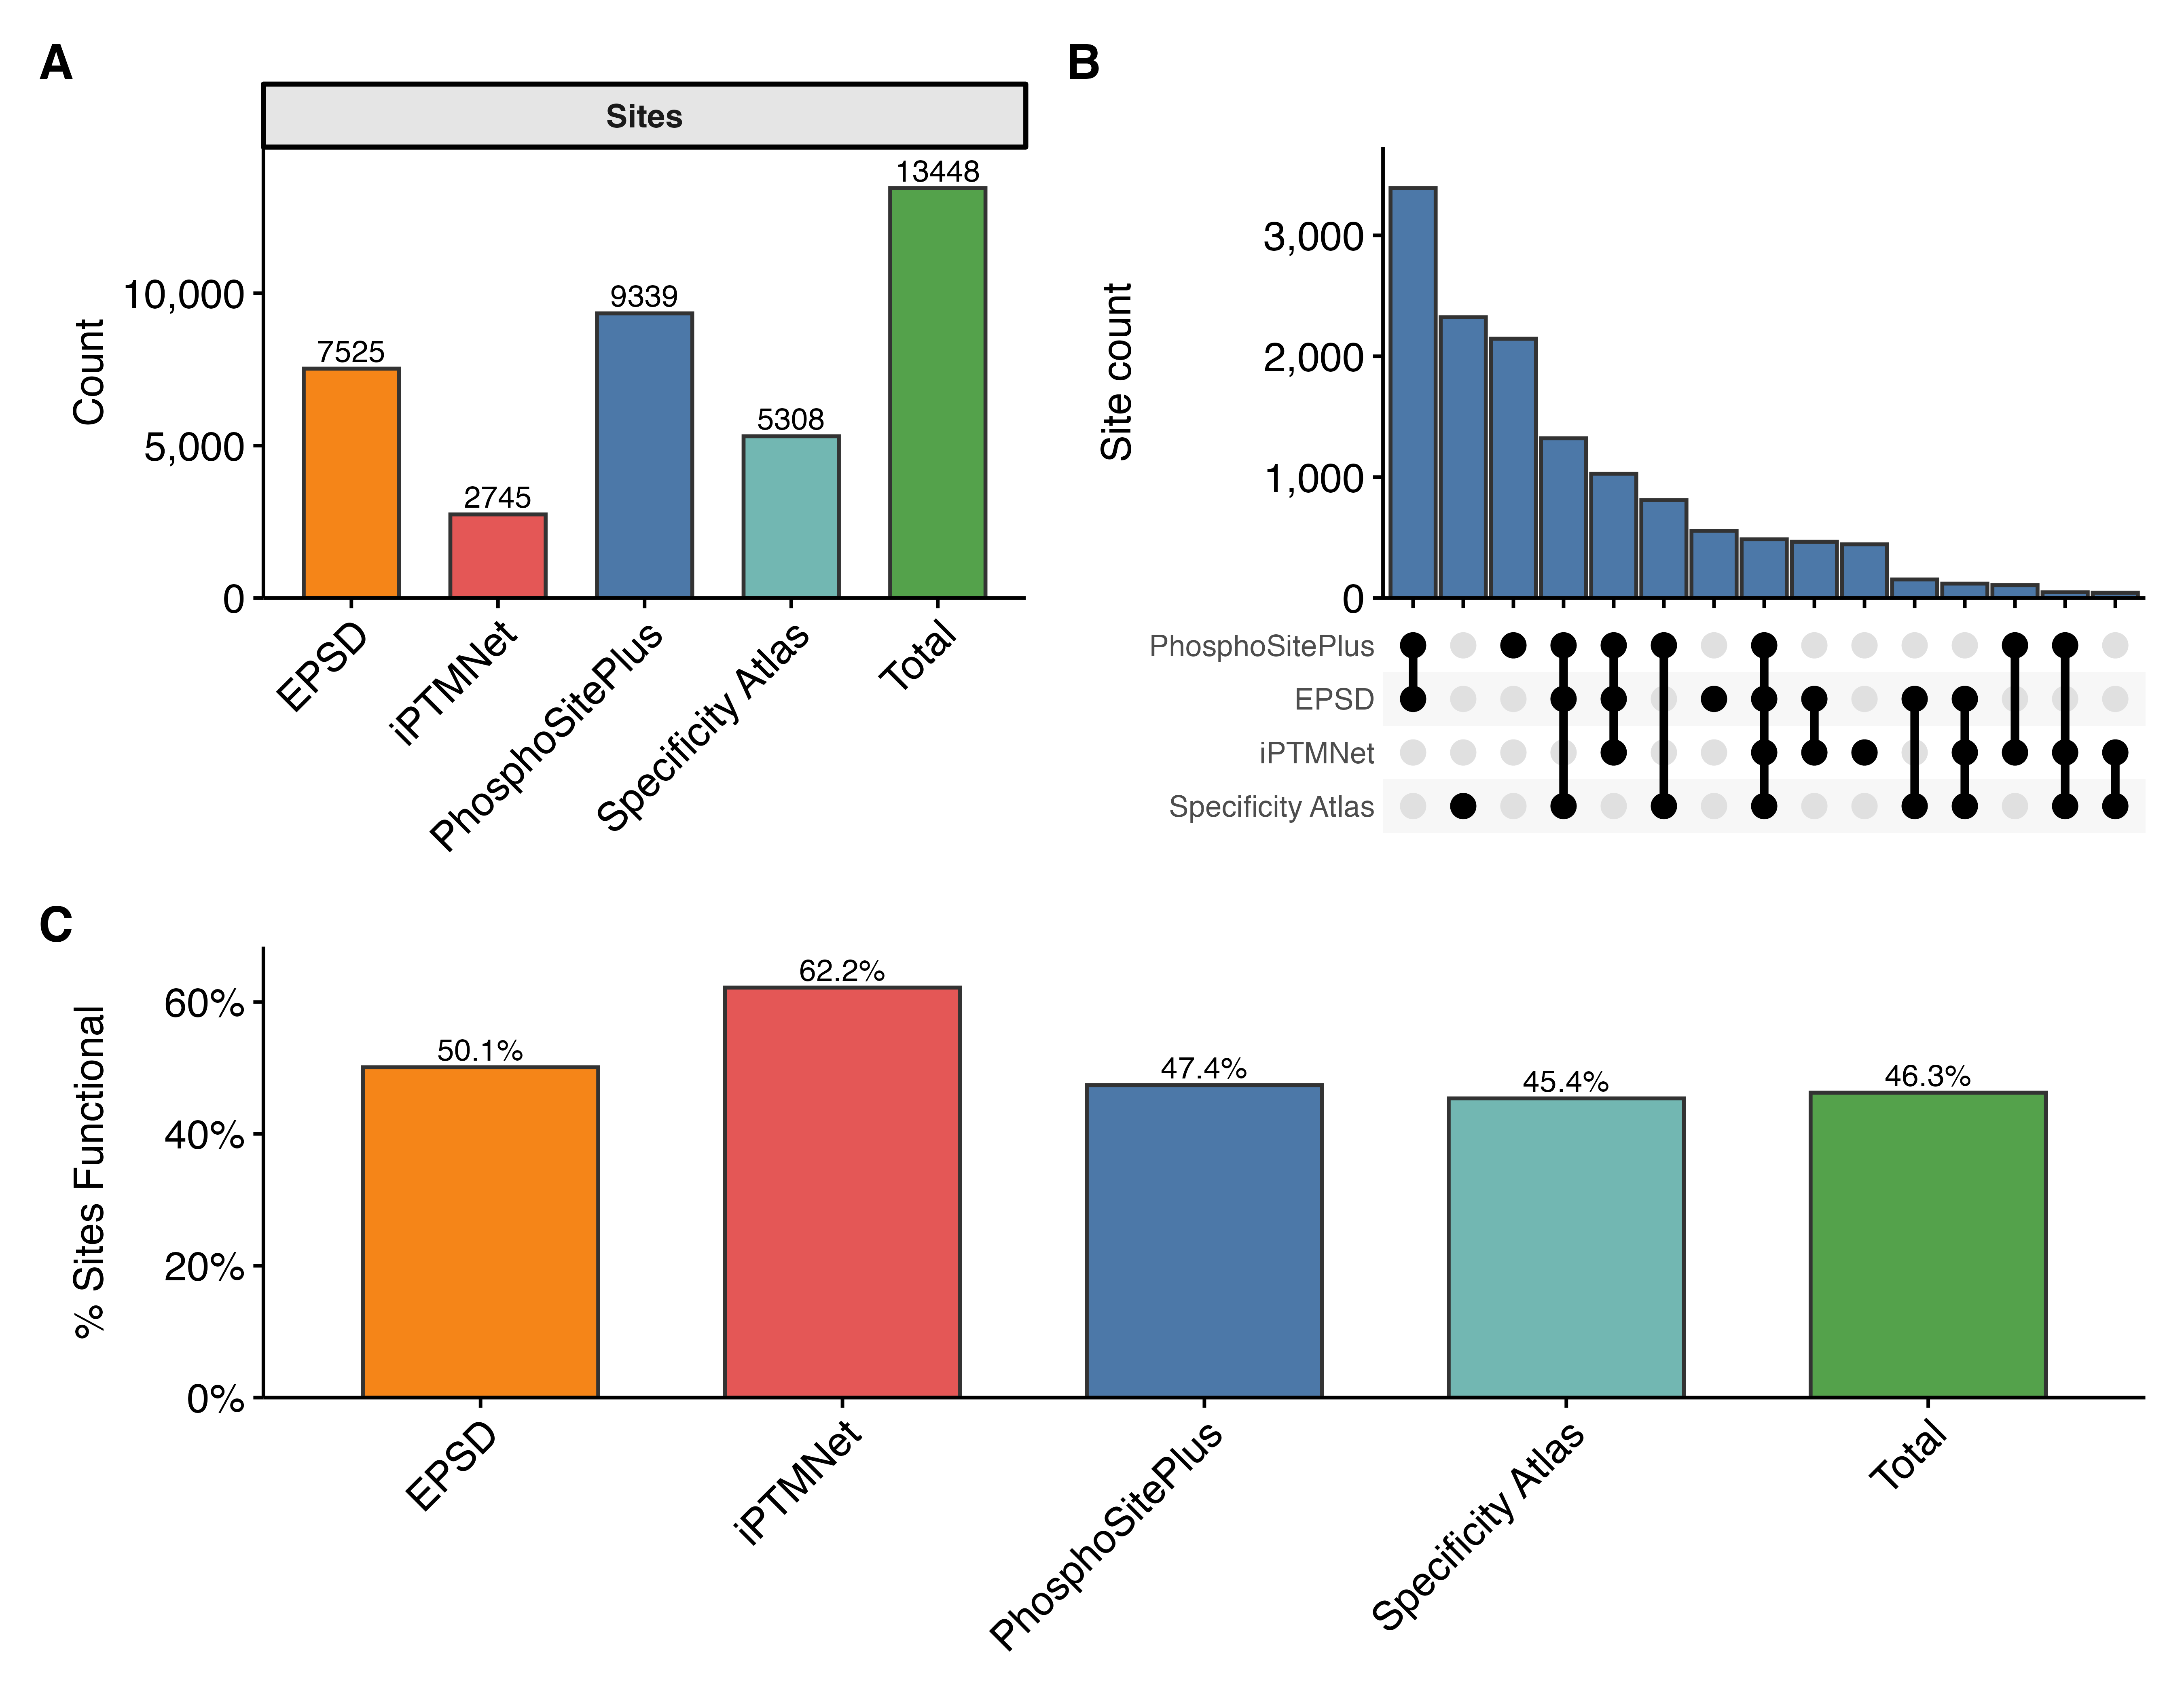
\includegraphics[keepaspectratio]{../figures/paper_figures/figS1.png}}

}

\caption{\label{sfig-1}\textbf{Comprehensive landscape and functional
density of integrated phosphosites.} A) Distribution of unique
phosphosite counts across individual database sources (PhosphoSitePlus,
EPSD, iPTMnet) and the predicted specificity atlas, alongside the
non-redundant integrated total. B) UpSet plot showing the intersection
of unique phosphosites across the four primary sources. While many sites
are unique to specific repositories, KinaseCanvas provides a unified
framework that highlights the substantial expansion provided by
integrating motif-based predictions. C) Percentage of phosphosites
within each source designated as `likely functional' (Ochoa functional
score \(\ge\) 0.5), demonstrating high functional density across both
curated and predicted datasets.}

\end{suppfig}%

Alt text: Three-panel figure showing phosphosite counts per database,
the percentage of functional sites across sources, and an UpSet plot
visualizing source overlaps.

\clearpage


\renewcommand\refname{References}
\bibliography{../refs/references.bib}



\end{document}
